%%%%%%%%%%%%%%%%%%%%%%%%%%%%%%%%%%%%%%%%%
% Beamer Presentation
% LaTeX Template
% Version 1.0 (10/11/12)
%
% This template has been downloaded from:
% http://www.LaTeXTemplates.com
%
% License:
% CC BY-NC-SA 3.0 (http://creativecommons.org/licenses/by-nc-sa/3.0/)
%
%%%%%%%%%%%%%%%%%%%%%%%%%%%%%%%%%%%%%%%%%

%----------------------------------------------------------------------------------------
%	PACKAGES AND THEMES
%----------------------------------------------------------------------------------------

%\documentclass[UTF8,aspectratio=169,14pt]{ctexbeamer}
\documentclass[UTF8,aspectratio=169]{ctexbeamer}
\usepackage{hyperref}
\hypersetup{
	colorlinks=true,
	linkcolor=red,
	anchorcolor=blue,
	citecolor=green
}

\mode<presentation> {
	
	% The Beamer class comes with a number of default slide themes
	% which change the colors and layouts of slides. Below this is a list
	% of all the themes, uncomment each in turn to see what they look like.
	
	%\usetheme{default}
	%\usetheme{AnnArbor}
	%\usetheme{Antibes}
	%\usetheme{Bergen}
	%\usetheme{Berkeley}
	%\usetheme{Berlin}
	%\usetheme{Boadilla}
	%\usetheme{CambridgeUS}
	%\usetheme{Copenhagen}
	%\usetheme{Darmstadt}
	%\usetheme{Dresden}
	%\usetheme{Frankfurt}
	%\usetheme{Goettingen}
	%\usetheme{Hannover}
	%\usetheme{Ilmenau}
	%\usetheme{JuanLesPins}
	%\usetheme{Luebeck}
	\usetheme{Madrid}
	%\usetheme{Malmoe}
	%\usetheme{Marburg}
	%\usetheme{Montpellier}
	%\usetheme{PaloAlto}
	%\usetheme{Pittsburgh}
	%\usetheme{Rochester}
	%\usetheme{Singapore}
	%\usetheme{Szeged}
	%\usetheme{Warsaw}
	
	% As well as themes, the Beamer class has a number of color themes
	% for any slide theme. Uncomment each of these in turn to see how it
	% changes the colors of your current slide theme.
	
	%\usecolortheme{albatross}
	%\usecolortheme{beaver}
	%\usecolortheme{beetle}
	%\usecolortheme{crane}
	%\usecolortheme{dolphin}
	%\usecolortheme{dove}
	%\usecolortheme{fly}
	%\usecolortheme{lily}
	%\usecolortheme{orchid}
	%\usecolortheme{rose}
	%\usecolortheme{seagull}
	%\usecolortheme{seahorse}
	%\usecolortheme{whale}
	%\usecolortheme{wolverine}
	
	%\setbeamertemplate{footline} % To remove the footer line in all slides uncomment this line
	%\setbeamertemplate{footline}[page number] % To replace the footer line in all slides with a simple slide count uncomment this line
	
	%\setbeamertemplate{navigation symbols}{} % To remove the navigation symbols from the bottom of all slides uncomment this line
}

\usepackage{graphicx} % Allows including images
\graphicspath{{./figs/}}
\usepackage{booktabs} % Allows the use of \toprule, \midrule and \bottomrule in tables
\usepackage{longtable}
\usepackage{listings}
\usepackage{xcolor}
\lstset{numbers=left, %设置行号位置
	numberstyle=\tiny, %设置行号大小
	keywordstyle=\color{blue}, %设置关键字颜色
	commentstyle=\color[cmyk]{1,0,1,0}, %设置注释颜色
	frame=single, %设置边框格式
	escapeinside=``, %逃逸字符(1左面的键),用于显示中文
	%breaklines, %自动折行
	extendedchars=false, %解决代码跨页时,章节标题,页眉等汉字不显示的问题
	xleftmargin=2em,xrightmargin=2em, aboveskip=1em, %设置边距
	tabsize=4, %设置tab空格数
	showspaces=false %不显示空格
}
% Fonts
% \usepackage{libertine}
% \setmonofont{Courier}
\setCJKsansfont[ItalicFont=Noto Serif CJK SC Black, BoldFont=Noto Sans CJK SC Black]{Noto Sans CJK SC}
\setmainfont[Ligatures={Common,TeX}]{Linux  Libertine O}
\setmonofont[SmallCapsFont={Latin Modern Mono Caps}]{Latin Modern Mono Light}
\setsansfont{Linux Biolinum O}

\logo{
\includegraphics[width=0.55cm,height=0.55cm]{../../thcs-logo.png}}

%----------------------------------------------------------------------------------------
%	TITLE PAGE
%----------------------------------------------------------------------------------------

\title[第3讲]{第3讲 :Virtual Machine Monitor} % The short title appears at the bottom of every slide, the full title is only on the title page
\subtitle{第一节:Overview }
\author{陈渝} % Your name
\institute[清华大学] % Your institution as it will appear on the bottom of every slide, may be shorthand to save space
{
	清华大学计算机系 \\ % Your institution for the title page
	\medskip
	\textit{yuchen@tsinghua.edu.cn} % Your email address
}
\date{\today} % Date, can be changed to a custom date


\begin{document}

\begin{frame}
\titlepage % Print the title page as the first slide
\end{frame}

%\begin{frame}
%\frametitle{提纲} % Table of contents slide, comment this block out to remove it
%\tableofcontents % Throughout your presentation, if you choose to use \section{} and \subsection{} commands, these will automatically be printed on this slide as an overview of your presentation
%\end{frame}
%
%%----------------------------------------------------------------------------------------
%%	PRESENTATION SLIDES
%%----------------------------------------------------------------------------------------
%
%%------------------------------------------------
%\section{第一节:课程概述} % Sections can be created in order to organize your presentation into discrete blocks, all sections and subsections are automatically printed in the table of contents as an overview of the talk
%%------------------------------------------------
%-------------------------------------------------
\begin{frame}[plain]
	\frametitle{Introduction}
	
	
	
	\begin{columns}
		
		\begin{column}{.4\textwidth}
			
			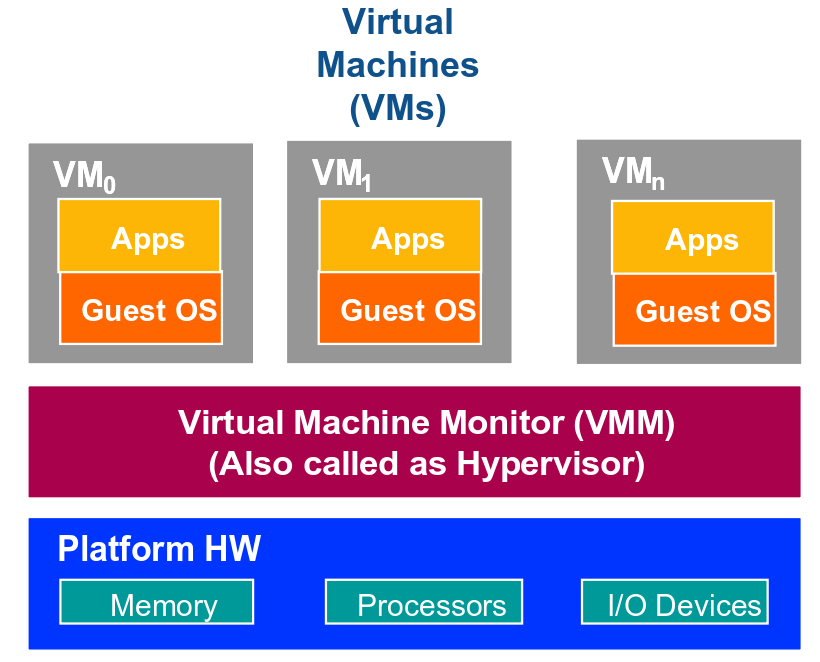
\includegraphics[width=1.\textwidth]{vmm-overview}
			
		\end{column}
		
		\begin{column}{.6\textwidth}
			
		
			\begin{block}{What is Virtualization}
				Virtualization is a term that refers to the abstraction of computer resources [wikipedia]
			\end{block}
		
			\begin{block}{Wisdom}
				All computer problems can be solved with another layer of redirection [Donald E. Knuth (高德纳), Stanford University]
			\end{block}

		\end{column}
		
		
	\end{columns}
	
	
\end{frame}

%-------------------------------------------------
\begin{frame}[plain]
	\frametitle{Introduction -- taxonomy}



	\begin{columns}

	\begin{column}{.3\textwidth}
	
	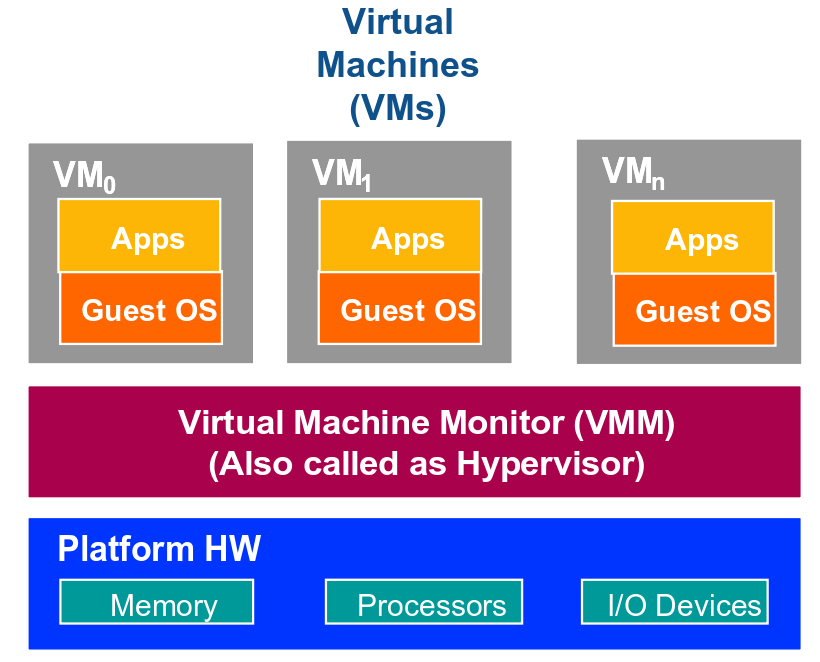
\includegraphics[width=1.\textwidth]{vmm-overview}
	
	\end{column}

	\begin{column}{.7\textwidth}
	
%	\Large
%    OS Structure	
%	\begin{itemize}
%	\item Simple kernel
%%	\item Monolithic kernel
%%	\item Micro kernel
%%	\item Exokernel
%%	\item VMM, etc...
%	\end{itemize}	

	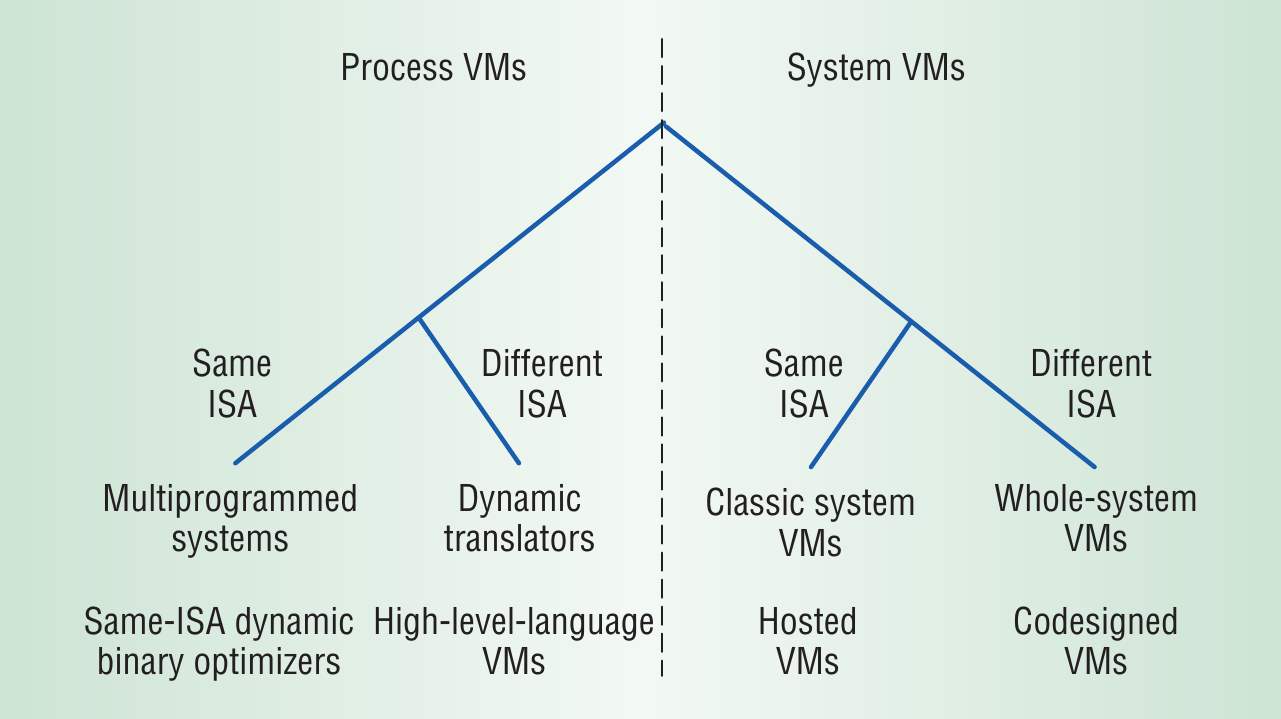
\includegraphics[width=1.\textwidth]{vm-taxonomy}
	
	\tiny	
	from James E.Smith,     IEEE computer Society2005	
	\end{column}
	
    
\end{columns}


\end{frame}

%-------------------------------------------------
\begin{frame}[plain]
	\frametitle{Introduction -- different layer of virtualization}
	
	
	
	\begin{columns}
		
		\begin{column}{.3\textwidth}
			
			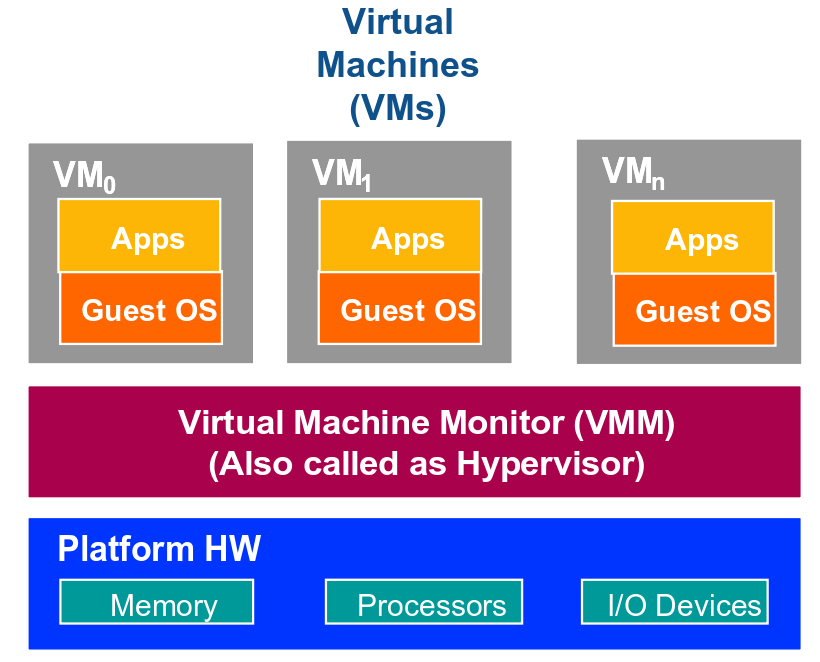
\includegraphics[width=1.\textwidth]{vmm-overview}
			
		\end{column}
		
		\begin{column}{.5\textwidth}
			
			%	\Large
			%    OS Structure	
			%	\begin{itemize}
			%	\item Simple kernel
			%%	\item Monolithic kernel
			%%	\item Micro kernel
			%%	\item Exokernel
			%%	\item VMM, etc...
			%	\end{itemize}	
			
			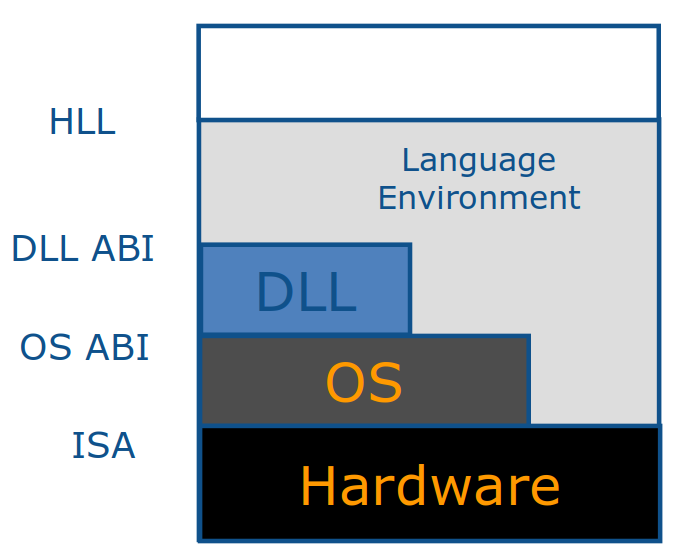
\includegraphics[width=1.\textwidth]{vm-layer}
			
			
		\end{column}
		
		
	\end{columns}
	
	
\end{frame}


%-------------------------------------------------
\begin{frame}[plain]
	\frametitle{Introduction -- VMM}
	
	
	
	\begin{columns}
		
		\begin{column}{.5\textwidth}
			
			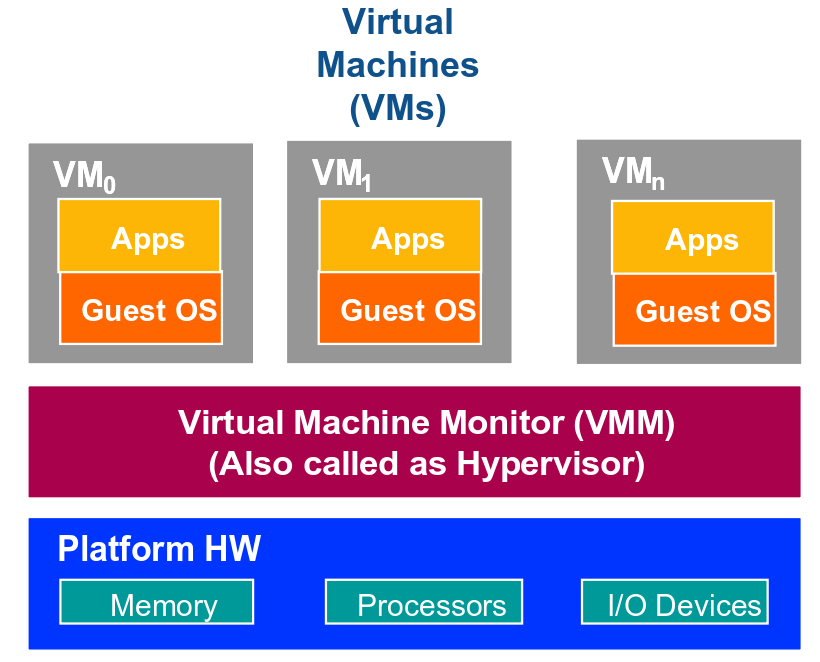
\includegraphics[width=1.\textwidth]{vmm-overview}
			
		\end{column}
		
		\begin{column}{.5\textwidth}
			
			\begin{block}{Virtual Machine Monitor, VMM}
	VMM transforms the single machine interface into the illusion of many. Each of these interfaces (virtual machines) is an efficient replica of the original computer system, complete with all of the processor instructions [Robert P. Goldberg, 1974]
			\end{block}
			
%			\begin{block}{Virtual Machine Monitor, VMM}
%				A virtual machine is implemented by adding software to an execution platform to give it the appearance of a different platform, or for that matter, to give the appearance of multiple platforms. [. E. Smith and Ravi Nair, “An Overview of Virtual Machine Architectures”.]
%			\end{block}
		\end{column}
		
		
	\end{columns}
	
	
\end{frame}

%-------------------------------------------------
\begin{frame}[plain]
	\frametitle{Introduction -- VMM}
	
	
	
	\begin{columns}
		
		\begin{column}{.5\textwidth}
			
			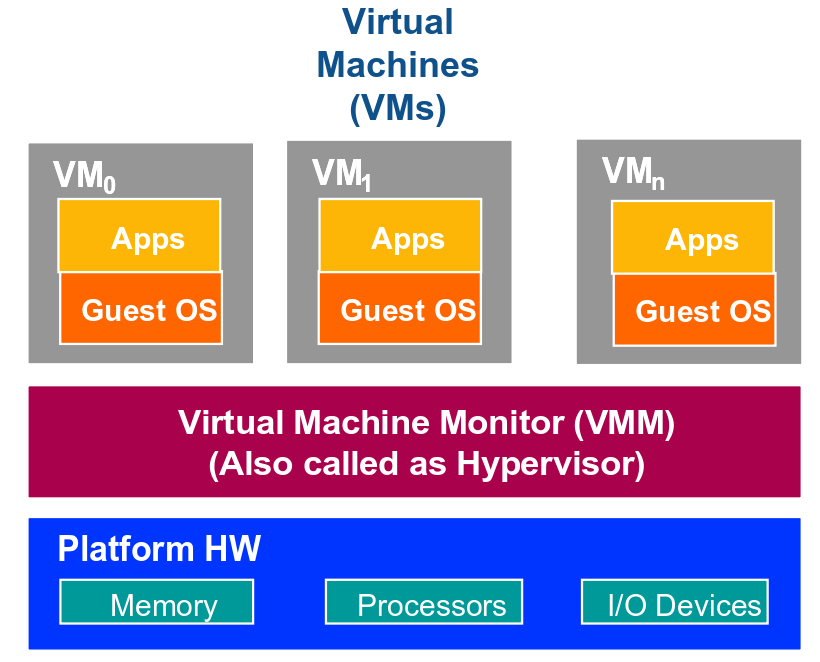
\includegraphics[width=1.\textwidth]{vmm-overview}
			
		\end{column}
		
		\begin{column}{.5\textwidth}
			
%			\begin{block}{Virtual Machine Monitor, VMM}
%				VMM transforms the single machine interface into the illusion of many. Each of these interfaces (virtual machines) is an efficient replica of the original computer system, complete with all of the processor instructions [Robert P. Goldberg, 1974]
%			\end{block}
			
			\begin{block}{Virtual Machine Monitor, VMM}
				A virtual machine is implemented by adding software to an execution platform to give it the appearance of a different platform, or for that matter, to give the appearance of multiple platforms. [J.E. Smith, “An Overview of Virtual Machine Architectures”]
			\end{block}
		\end{column}
		
		
	\end{columns}
	
	
\end{frame}


%-------------------------------------------------
\begin{frame}[plain]
	\frametitle{Introduction -- Why VMM?}
	
	
	
	\begin{columns}
		
		\begin{column}{.5\textwidth}
			
			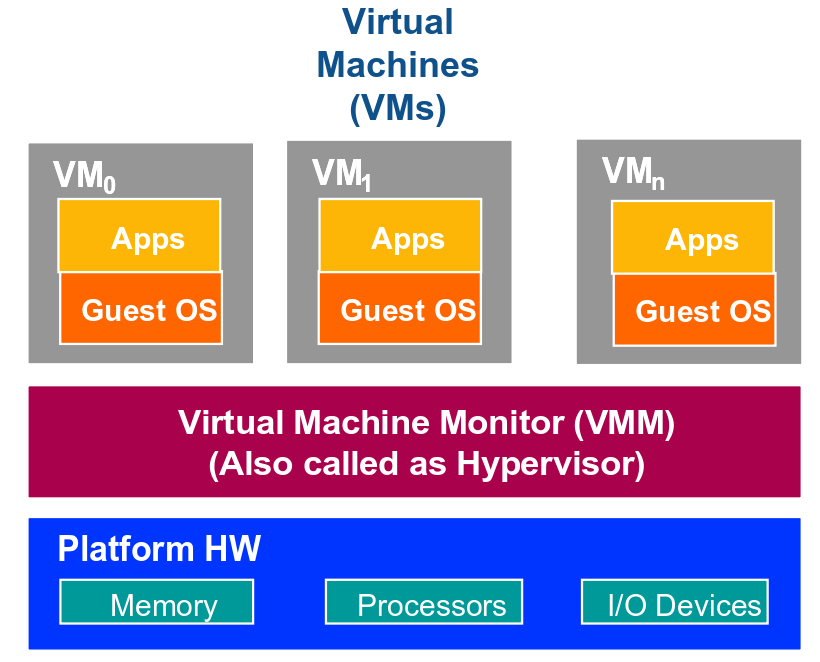
\includegraphics[width=1.\textwidth]{vmm-overview}
			
		\end{column}
		
		\begin{column}{.5\textwidth}
		
		Before there were data centers... 
		\begin{itemize}
			\item Many early commercial computers were mainframes
			\item powerful computation, highly reliable, extensive I/O capabilities
			\item for computing/data-intensive  apps 
			
		\end{itemize} 	
        IBM	System/360 hardware and CP/CMS system software: Virtualizable Architecture
		\end{column}
		
		
	\end{columns}
		
\end{frame}


%-------------------------------------------------
\begin{frame}[plain]
	\frametitle{Introduction -- Why VMM?}
	
	
	
	\begin{columns}
		
		\begin{column}{.5\textwidth}
			
			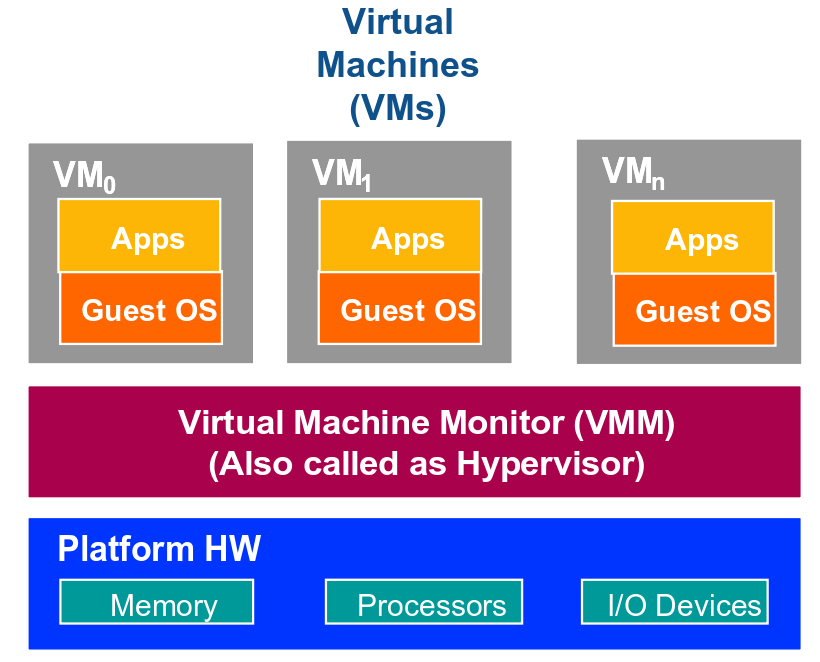
\includegraphics[width=1.\textwidth]{vmm-overview}
			
		\end{column}
		
		\begin{column}{.5\textwidth}
			
			Now there were data centers... 
			\begin{itemize}
				\item Many computers were servers connected in the world.
				\item powerful computation, highly reliable, extensive I/O capabilities
				\item for computing/data-intensive apps 

				
			\end{itemize} 	
			 x86/ARM and Linux/KVM, vmware, xen, etc. system software: Virtualizable Architecture
		\end{column}
		
		
	\end{columns}
	
\end{frame}


%-------------------------------------------------
\begin{frame}[plain]
	\frametitle{Introduction -- Essential characteristics of VMM}
	
	
	
	\begin{columns}
		
		\begin{column}{.5\textwidth}
			
			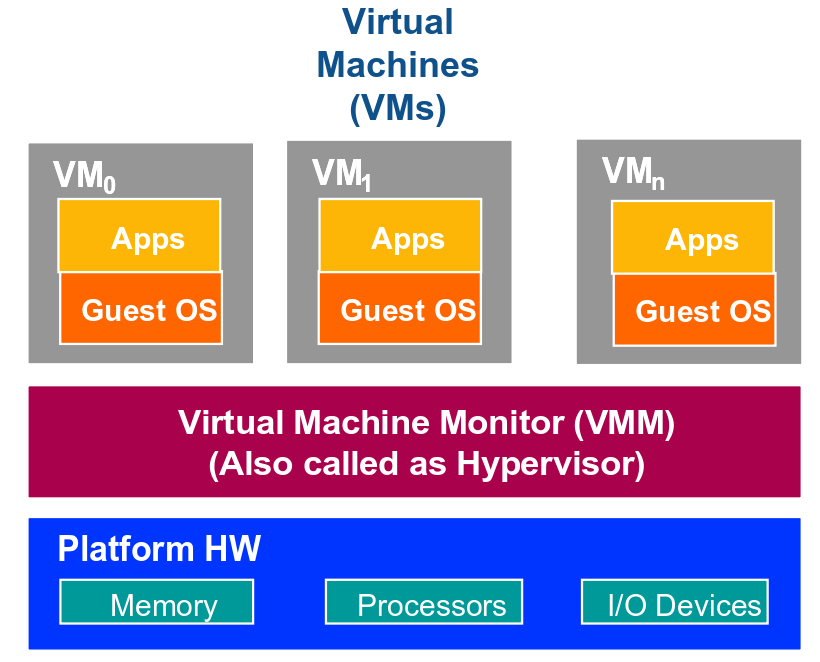
\includegraphics[width=1.\textwidth]{vmm-overview}
			
		\end{column}
		
		\begin{column}{.5\textwidth}
			
	     \begin{itemize}
			\item Equivalence: Essentially identical virtual platform, except
			\begin{itemize}
				\item Differences caused by the availability of system resources. e.g. memory size

			\end{itemize} \pause
			
			\item Isolation, or resource control 
			\begin{itemize}
				\item VMM is in complete control of system resources
				
			\end{itemize} \pause
			
			\item Efficiency
			\begin{itemize}
				\item At worst only minor decreases in speed
				\item speed $>>$ emulators, software interpreters (simulators)
				
			\end{itemize}
		
     	\end{itemize}	
	
		\end{column}
		
		
	\end{columns}
	
	
\end{frame}

%-------------------------------------------------
\begin{frame}[plain]
	\frametitle{How VMM works }
	
	
	
	\begin{columns}
		
		\begin{column}{.3\textwidth}
			
			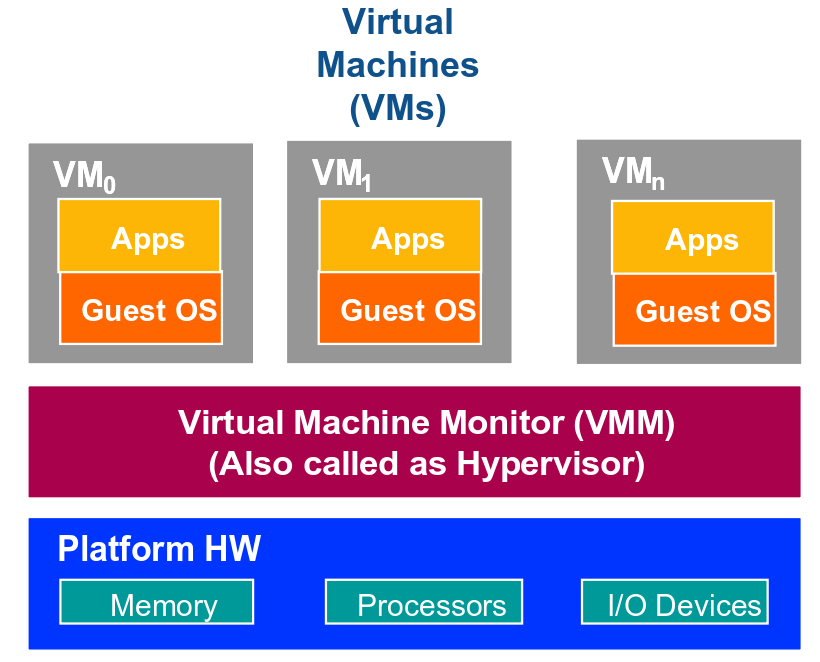
\includegraphics[width=1.\textwidth]{vmm-overview}
			
		\end{column}
		
		\begin{column}{.7\textwidth}
			
			Start with a “simpler” question:  how do (regular) machines work?	

			\centering
			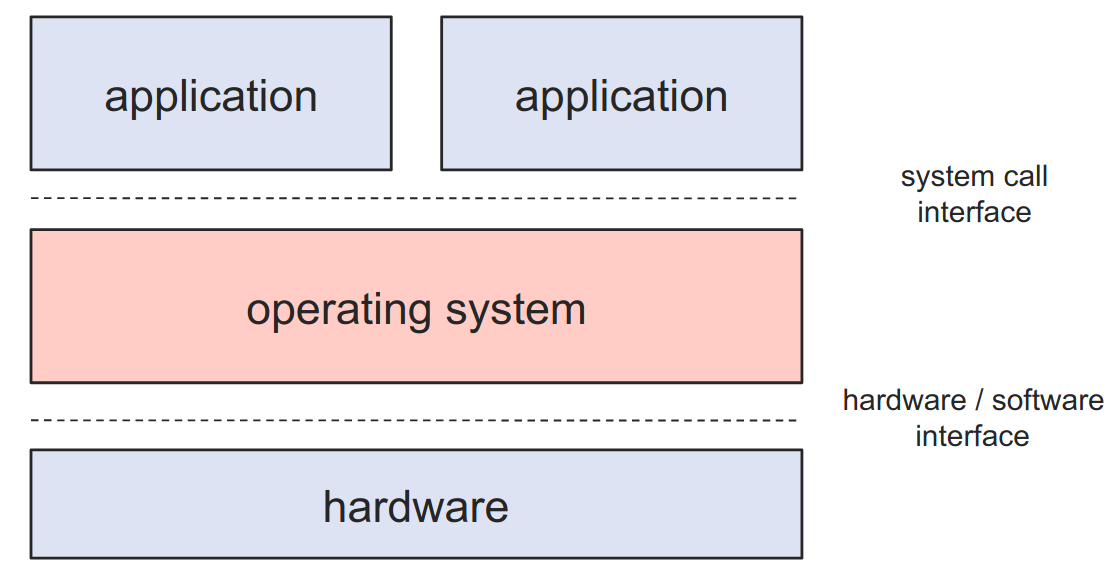
\includegraphics[width=.7\textwidth]{os-do-work}	
			
			\begin{itemize}
				\item What is computer hardware? (CPU, MEM, IO)
				\item What is an OS? 
				\item What‘s an application? (relies on the system call interface)
				
			\end{itemize} 
				
		\end{column}
		
		
	\end{columns}
	
	
\end{frame}


%-------------------------------------------------
\begin{frame}[plain]
	\frametitle{How VMM works }
	
	
	
	\begin{columns}
		
		\begin{column}{.3\textwidth}
			
			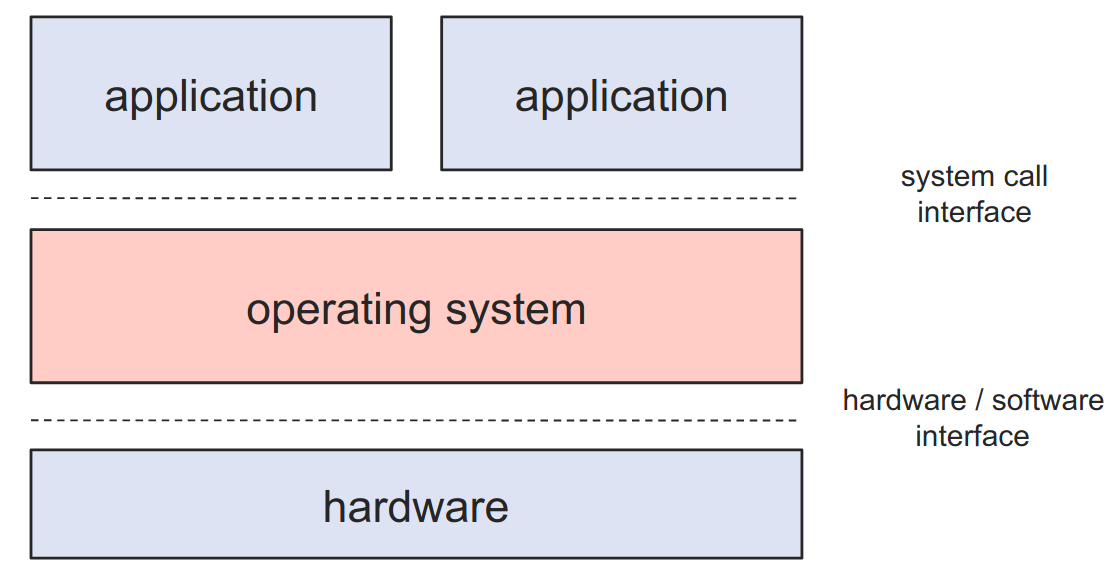
\includegraphics[width=1.\textwidth]{os-do-work}
			
		\end{column}
		
		\begin{column}{.7\textwidth}
			
			Start with a “simpler” question:  how do (regular) machines work?	
			
			\centering
			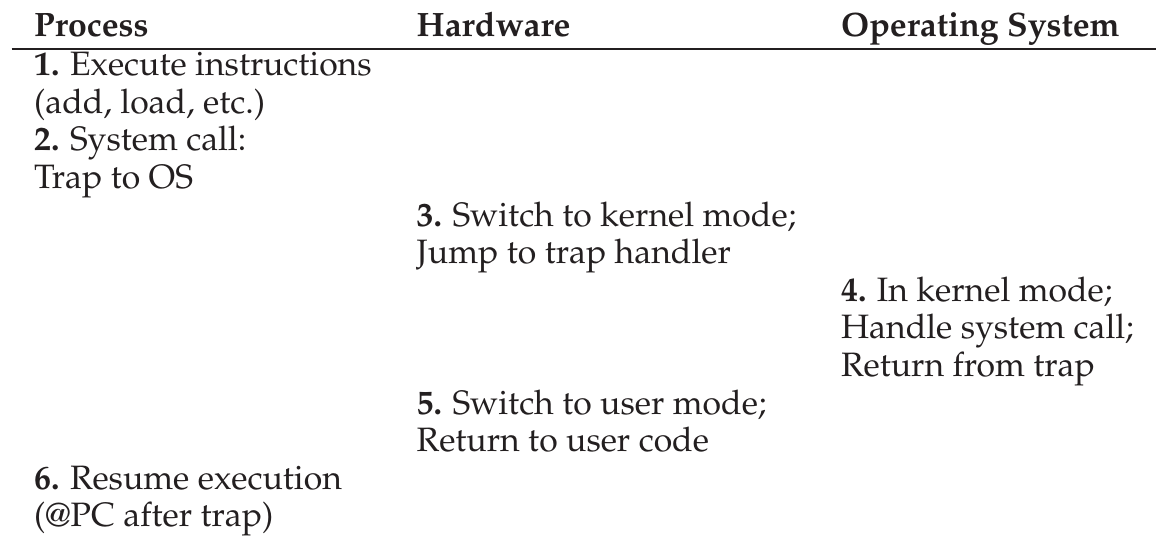
\includegraphics[width=1.\textwidth]{exec-syscall}	
			
			Executing a System Call
			
%			\begin{itemize}
%				\item What is computer hardware? (CPU, MEM, IO)
%				\item What is an OS? 
%				\item What’s an application? (relies on the system call interface)
%				
%			\end{itemize} 
			
		\end{column}
		
		
	\end{columns}
	
	
\end{frame}

%-------------------------------------------------
\begin{frame}[plain]
	\frametitle{How VMM works -- CPU}
	
	
	
	\begin{columns}
		
		\begin{column}{.3\textwidth}
			
			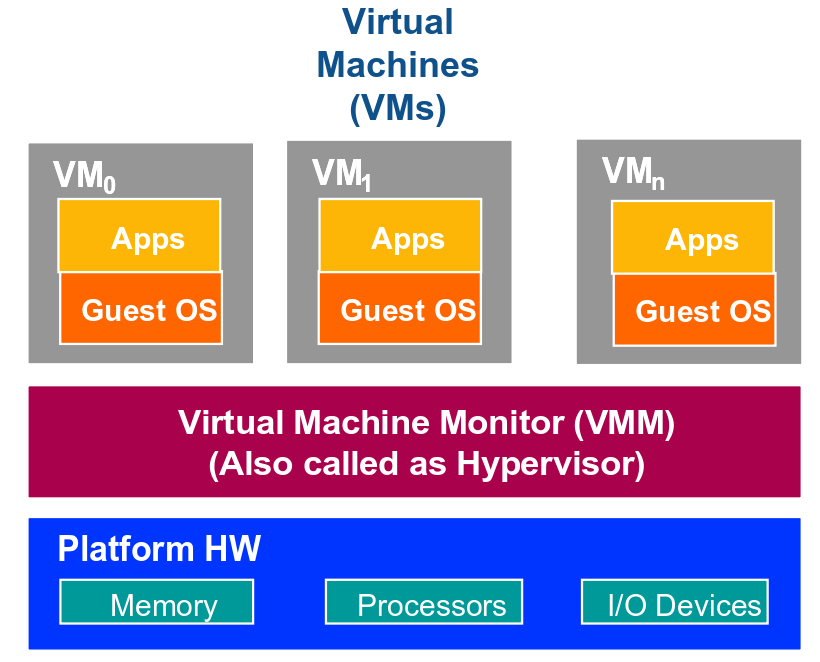
\includegraphics[width=1.\textwidth]{vmm-overview}
			
		\end{column}
		
		\begin{column}{.7\textwidth}
			
			What if we run the Linux/Windows kernel as a user-level program?	
			
			\centering
			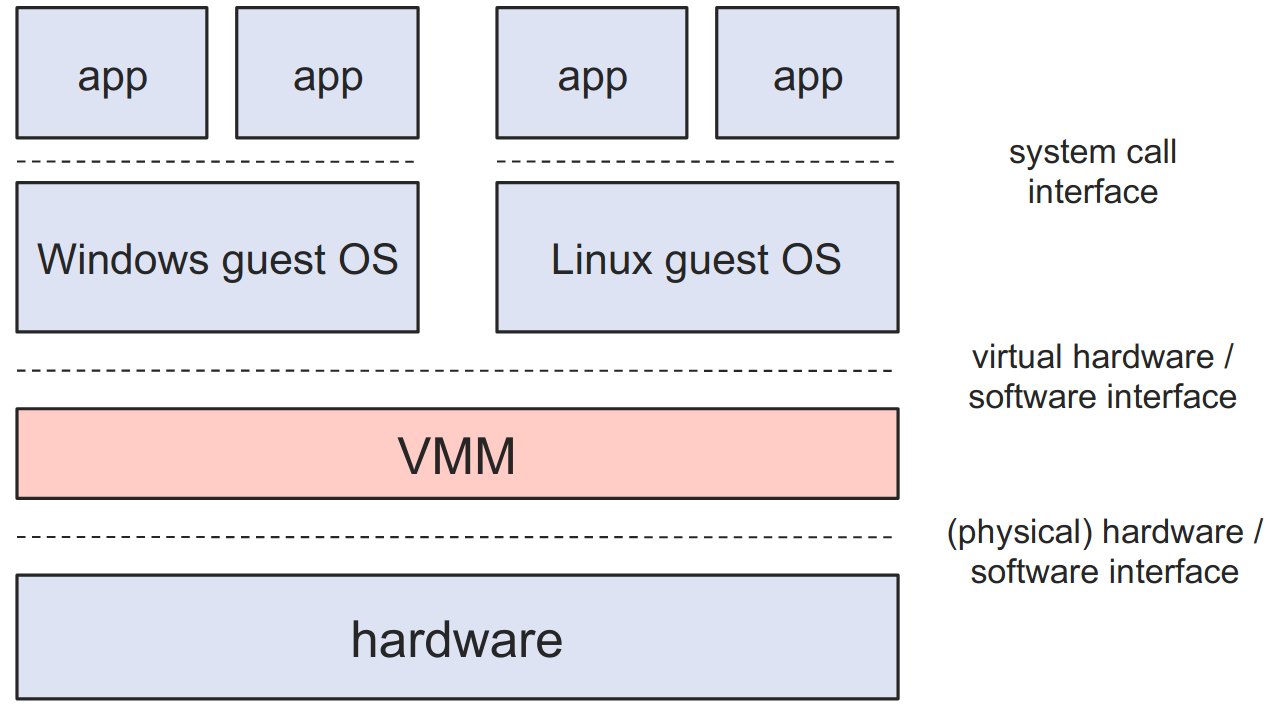
\includegraphics[width=.7\textwidth]{vmm-do-work}	
			
			\begin{itemize}
				\item What happens when Linux issues a sensitive instruction?
				\item What (virtual) hardware devices should Windows see?  
				\item How do you prevent apps running on Linux from hurting Linux?
				
			\end{itemize} 
			
		\end{column}
		
		
	\end{columns}
	
	
\end{frame}


%-------------------------------------------------
\begin{frame}[plain]
	\frametitle{How VMM works  -- CPU}
	
	
	
	\begin{columns}
		
		\begin{column}{.3\textwidth}
			
			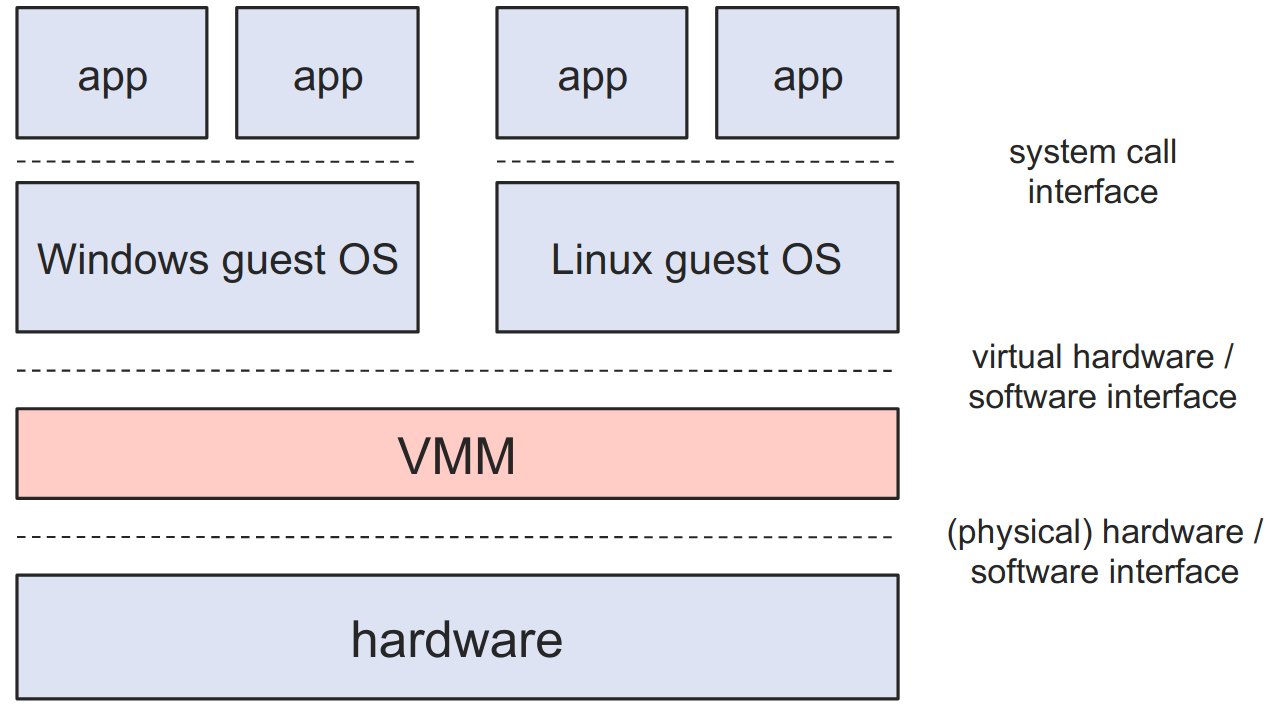
\includegraphics[width=1.\textwidth]{vmm-do-work}
			
		\end{column}
		
		\begin{column}{.7\textwidth}
			
			What if we run the Linux/Windows kernel as a user-level program?	
			
			\centering
			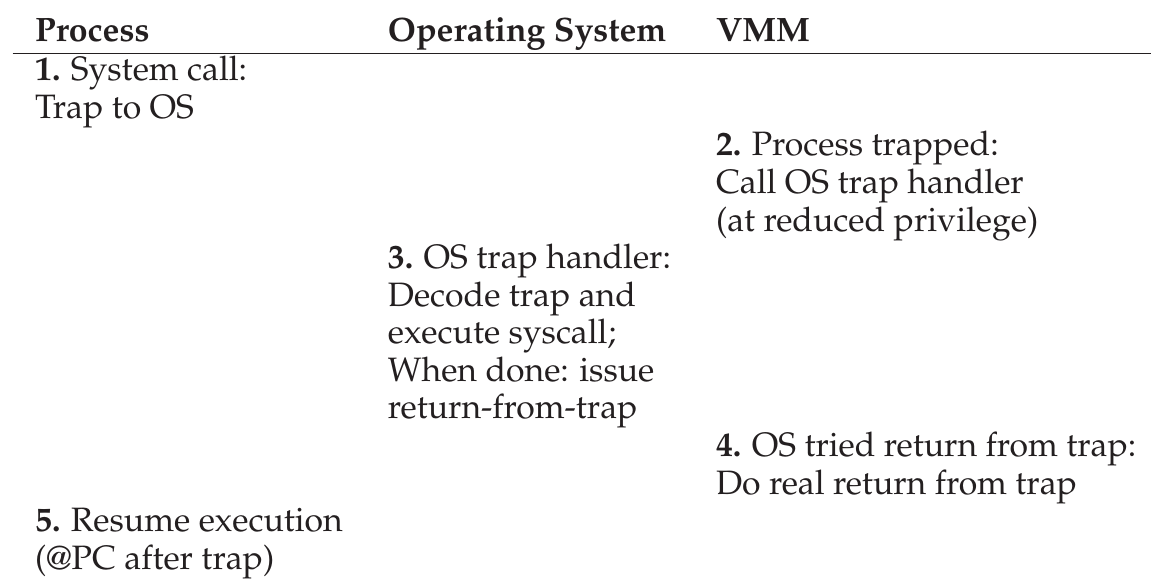
\includegraphics[width=1.\textwidth]{exec-syscall-in-vmm}	
			
			System Call Flow with Virtualization
			
			
		\end{column}
		
		
	\end{columns}
	
	
\end{frame}

%-------------------------------------------------
\begin{frame}[plain]
	\frametitle{How VMM works  -- CPU}
	
	
	
	\begin{columns}
		
		\begin{column}{.25\textwidth}
			
			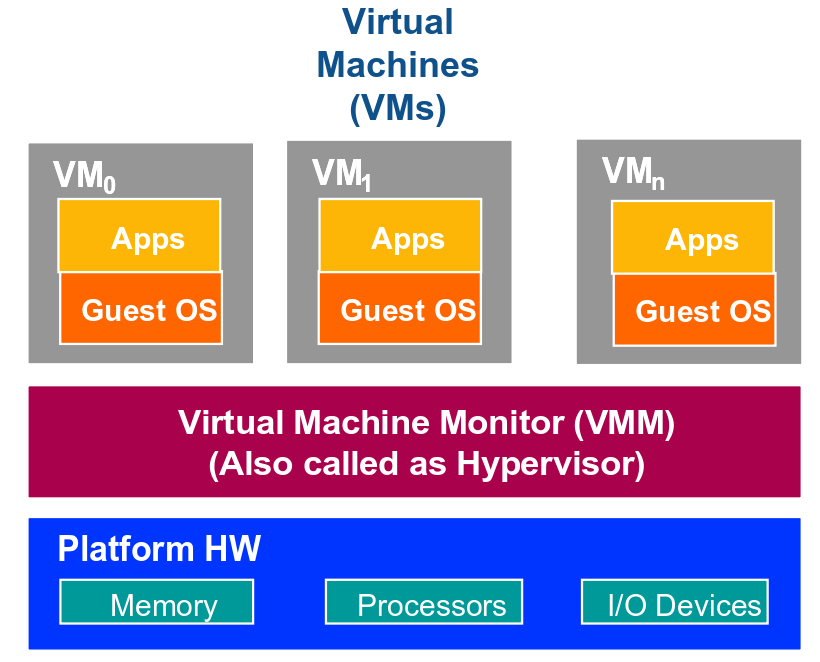
\includegraphics[width=1.\textwidth]{vmm-overview}
			
		\end{column}
		
		\begin{column}{.75\textwidth}
			
			What if we run the Linux/Windows kernel as a user-level program?	
			
			\centering
			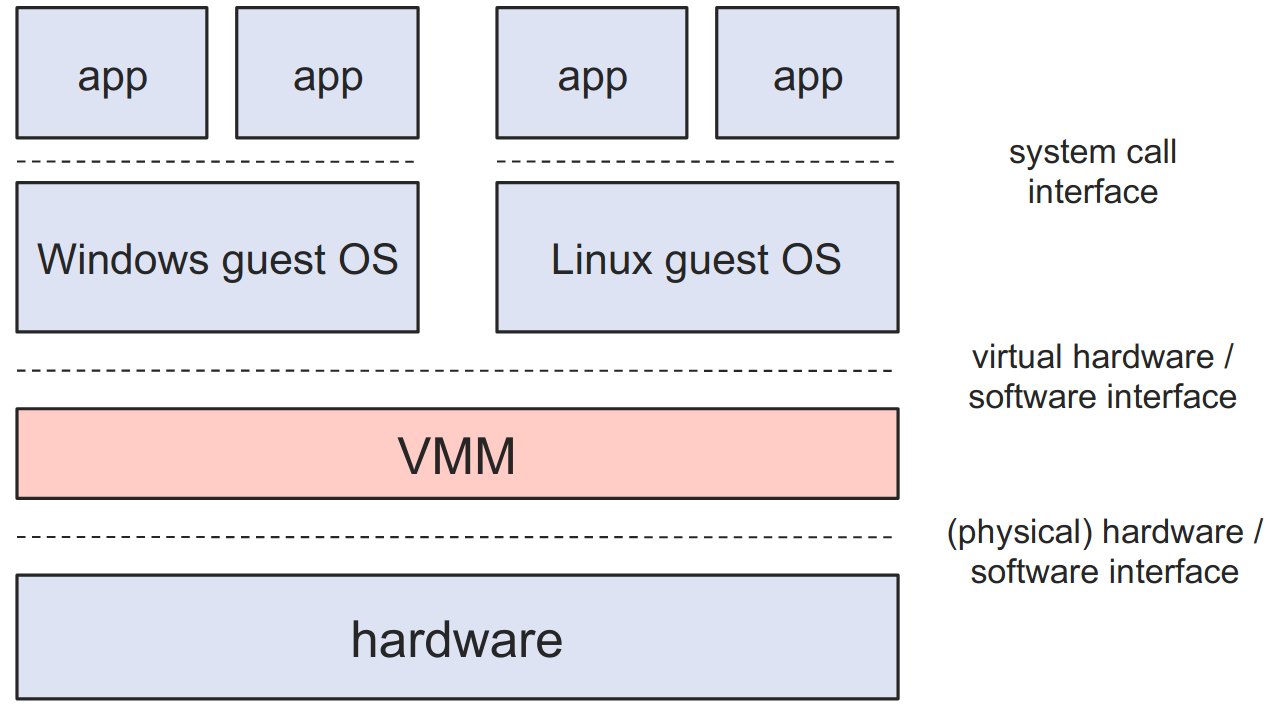
\includegraphics[width=.6\textwidth]{vmm-do-work}	
			\begin{flushleft}
			Answer: rely on CPU to trap sensitive instructions and hand off to VMM
			\end{flushleft}
			\begin{itemize}
				\item VMM emulates the effect of sensitive instruction on the virtual hardware that it provides to its guest OSs 
				\item VMM provides a virtual HW/SW interface to guest OSs by trapping and emulating sensitive instructions 
				
			\end{itemize} 
			
		\end{column}
		
		
	\end{columns}
	
	
\end{frame}



%-------------------------------------------------
\begin{frame}[plain]
	\frametitle{How VMM works  -- CPU}
	
	
	
	\begin{columns}
		
		\begin{column}{.25\textwidth}
			
			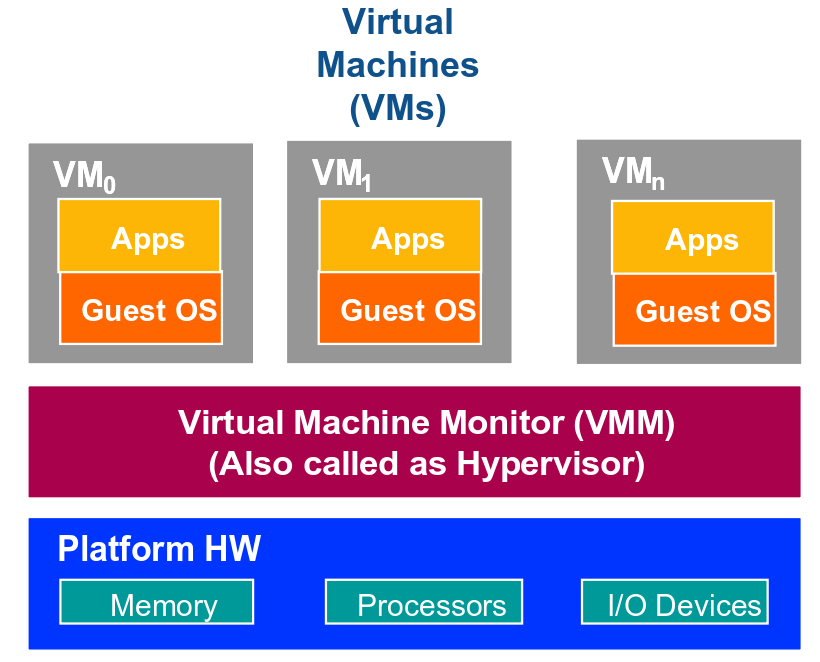
\includegraphics[width=1.\textwidth]{vmm-overview}
			
		\end{column}
		
		\begin{column}{.75\textwidth}
			
			What if we run the Linux/Windows kernel as a user-level program?	
			
			\centering
			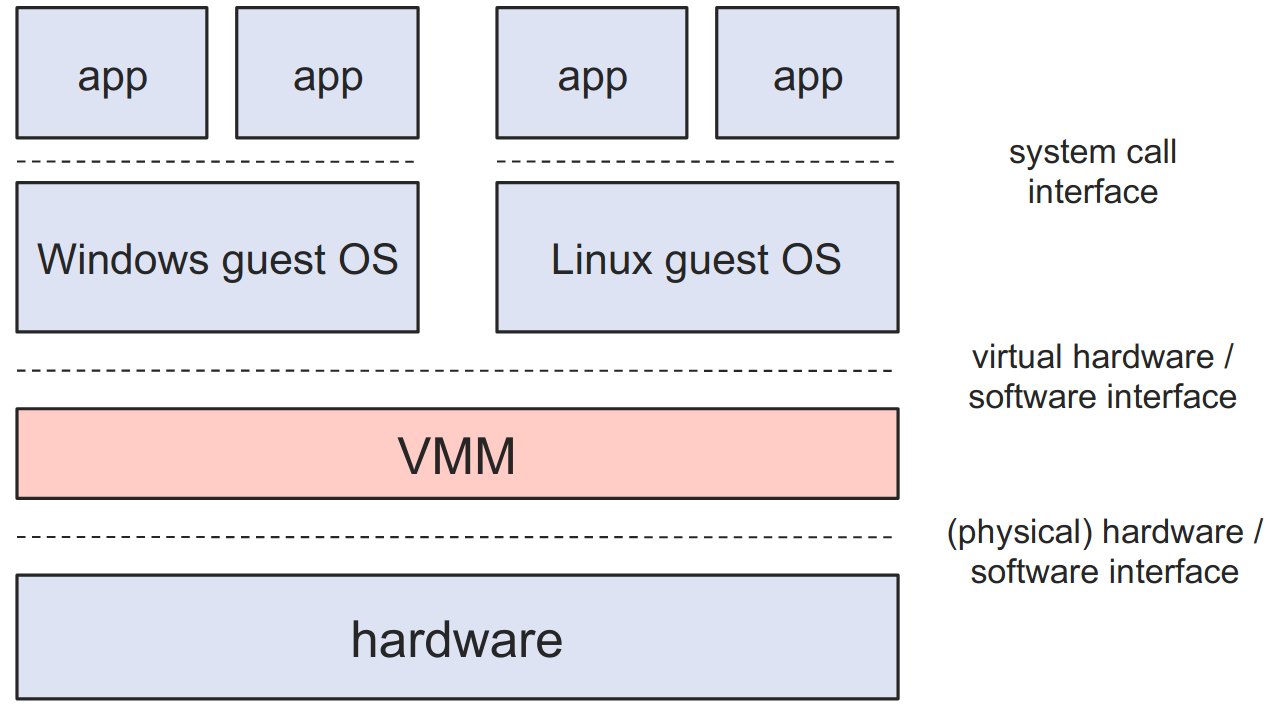
\includegraphics[width=.6\textwidth]{vmm-do-work}	
			\begin{flushleft}
				Goldberg (1974):  two classes of instructions 
			\end{flushleft}
			\begin{itemize}
				\item privileged instructions:   those that trap when CPU is in user-mode  
				\item sensitive instructions:   those that modify hardware configuration or resources, and those whose behavior depends on HW configuration 
				
			\end{itemize} 
			
		\end{column}
		
		
	\end{columns}
	
	
\end{frame}


%-------------------------------------------------
\begin{frame}[plain]
	\frametitle{How VMM works  -- CPU}
	
	
	
	\begin{columns}
		
		\begin{column}{.25\textwidth}
			
			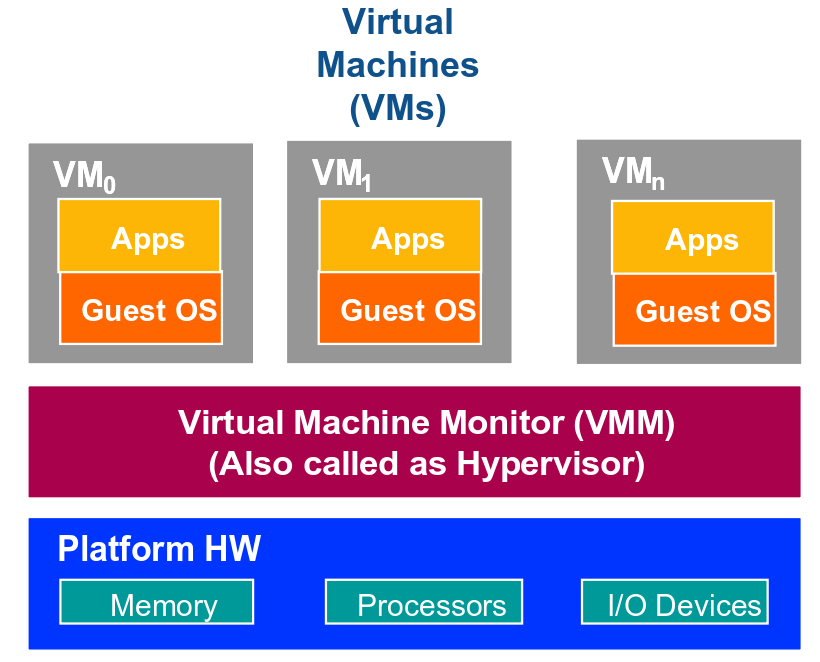
\includegraphics[width=1.\textwidth]{vmm-overview}
			
		\end{column}
		
		\begin{column}{.75\textwidth}
			
			What if we run the Linux/Windows kernel as a user-level program?	
			
			\centering
			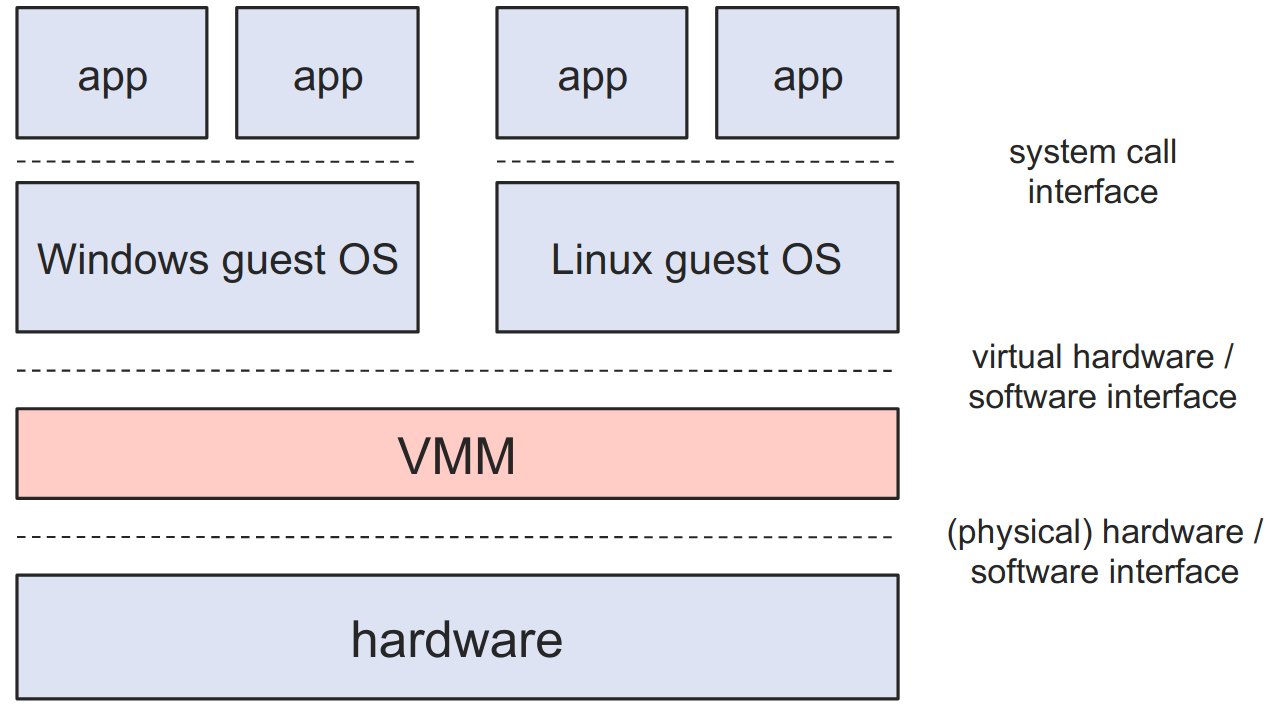
\includegraphics[width=.6\textwidth]{vmm-do-work}	
			\begin{flushleft}
				\textbf{A VMM can be constructed efficiently and safely if the set of sensitive instructions is a subset of the set of privileged instructions.}
			\end{flushleft}
%			\begin{itemize}
%				\item privileged instructions:   those that trap when CPU is in user-mode  
%				\item sensitive instructions:   those that modify hardware configuration or resources, and those whose behavior depends on HW configuration 
%				
%			\end{itemize} 
			
		\end{column}
		
		
	\end{columns}
	
	
\end{frame}



%-------------------------------------------------
\begin{frame}[plain]
	\frametitle{How VMM works -- memory}
	
	
	
	\begin{columns}
		
		\begin{column}{.25\textwidth}
			
			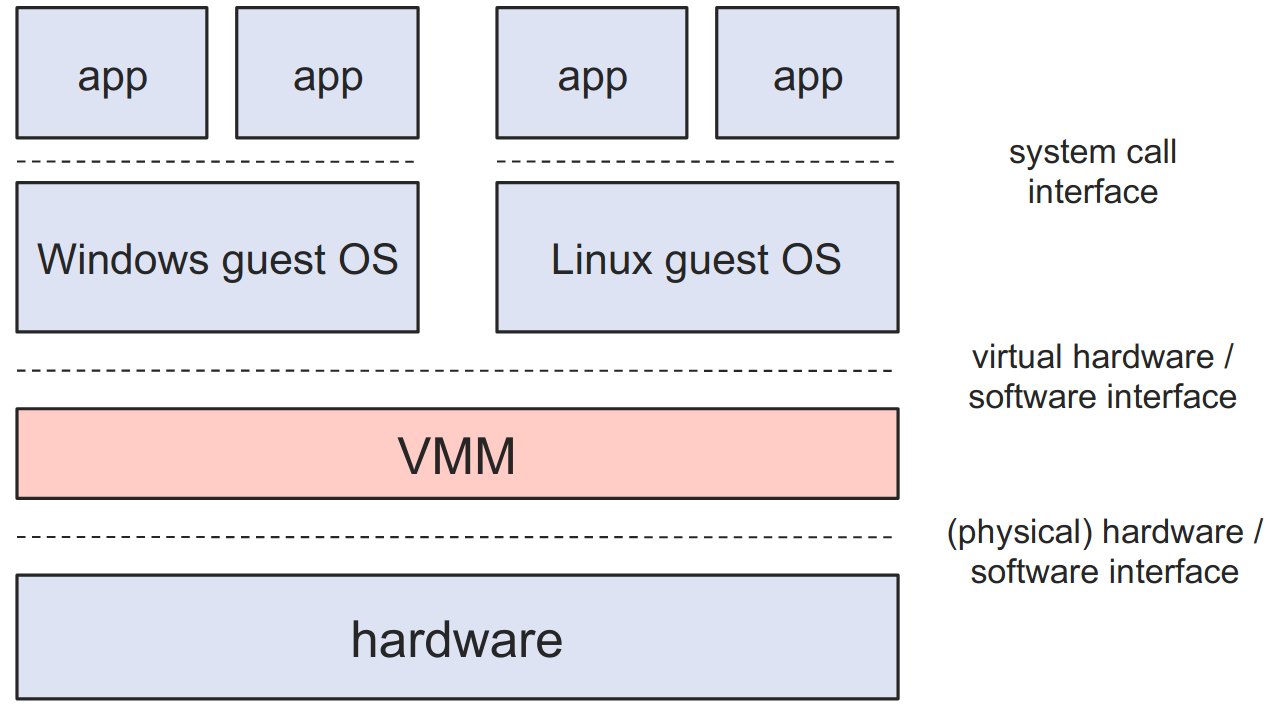
\includegraphics[width=1.\textwidth]{vmm-do-work}
			
		\end{column}
		
		\begin{column}{.75\textwidth}
			
%			What if we run the Linux/Windows kernel as a user-level program?	
			
			\centering
			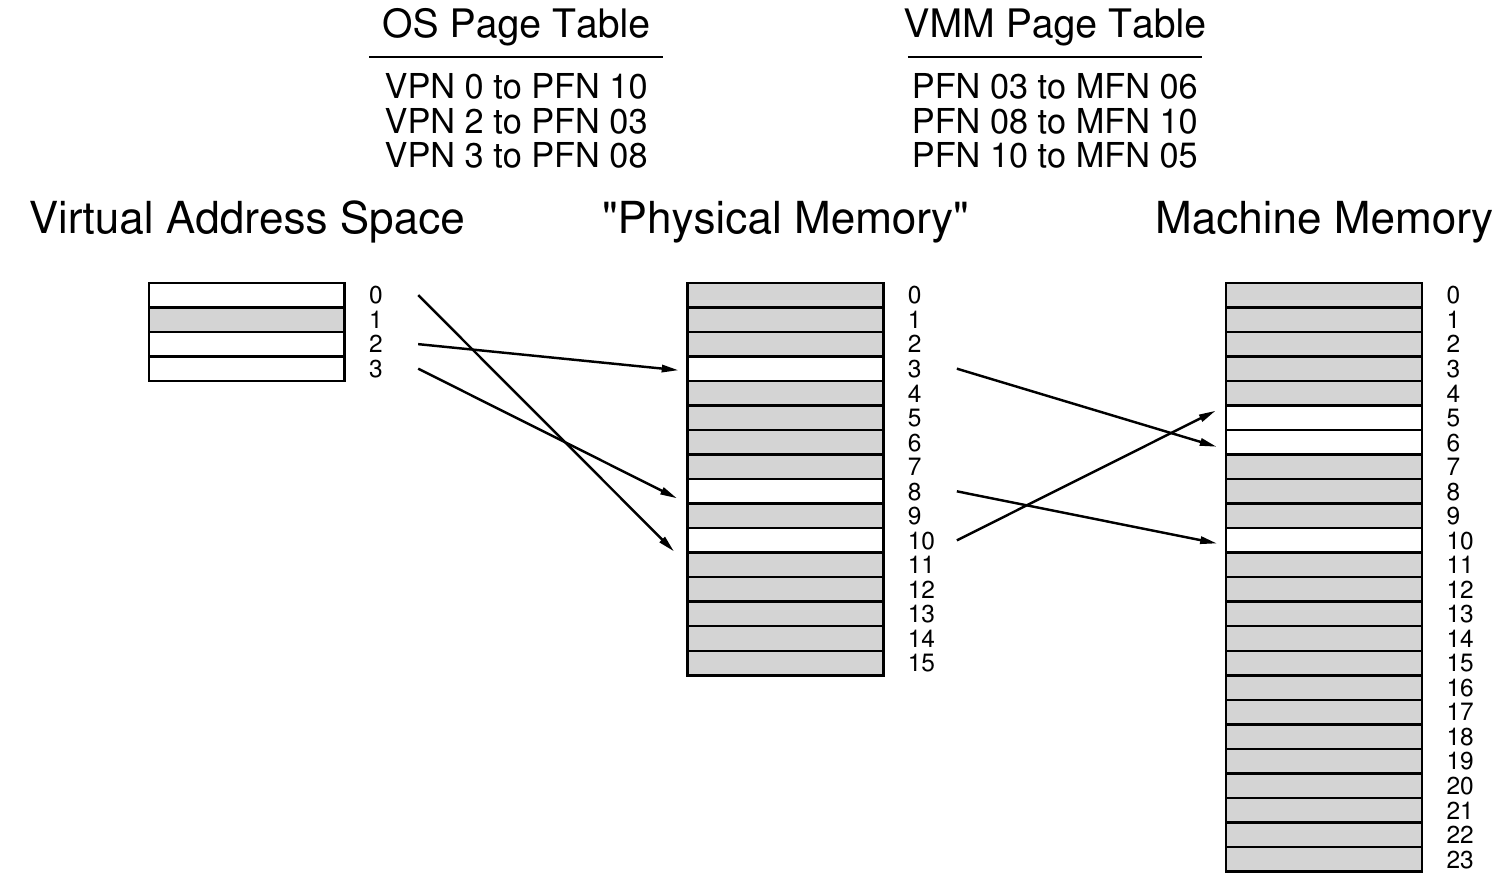
\includegraphics[width=1.\textwidth]{vmm-address-space}	
%			\begin{flushleft}
				VMM Memory Virtualization
%			\end{flushleft}

			
		\end{column}
		
		
	\end{columns}
	
	
\end{frame}


%-------------------------------------------------
\begin{frame}[plain]
	\frametitle{How VMM works -- memory}
	
	
	
	\begin{columns}
		
		\begin{column}{.25\textwidth}
			
			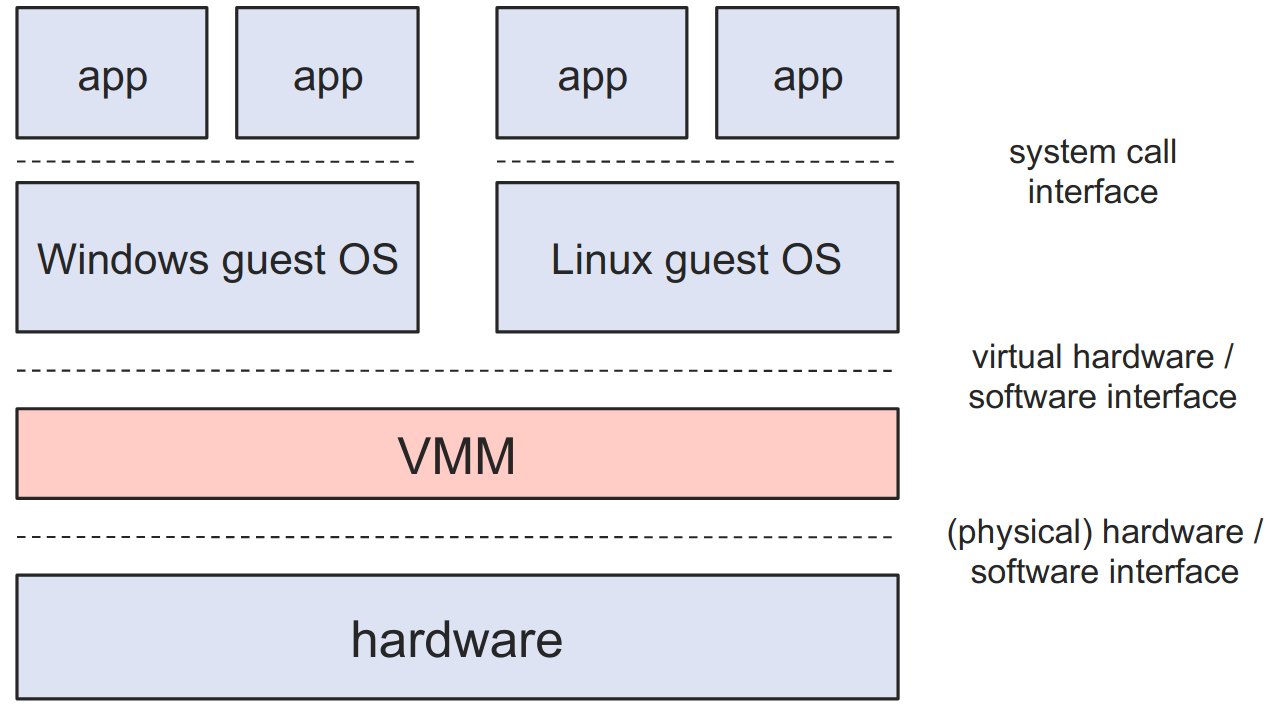
\includegraphics[width=1.\textwidth]{vmm-do-work}
			
		\end{column}
		
		\begin{column}{.75\textwidth}
			
			%			What if we run the Linux/Windows kernel as a user-level program?	
			
			\centering
			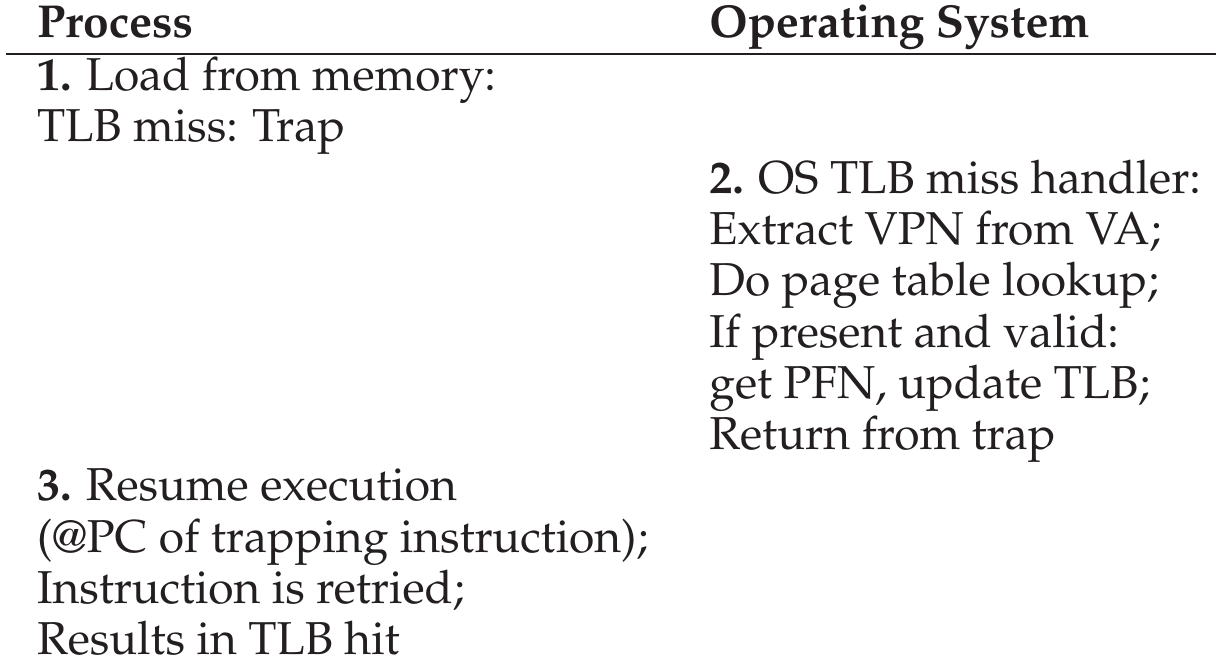
\includegraphics[width=.9\textwidth]{os-tlbmiss}	
			%			\begin{flushleft}
			
			\textbf{TLB Miss Flow without Virtualization}
			
			%			\end{flushleft}
			
			
		\end{column}
		
		
	\end{columns}
	
	
\end{frame}


%-------------------------------------------------
\begin{frame}[plain]
	\frametitle{How VMM works -- memory}
	
	
	
	\begin{columns}
		
		\begin{column}{.2\textwidth}
			\centering
			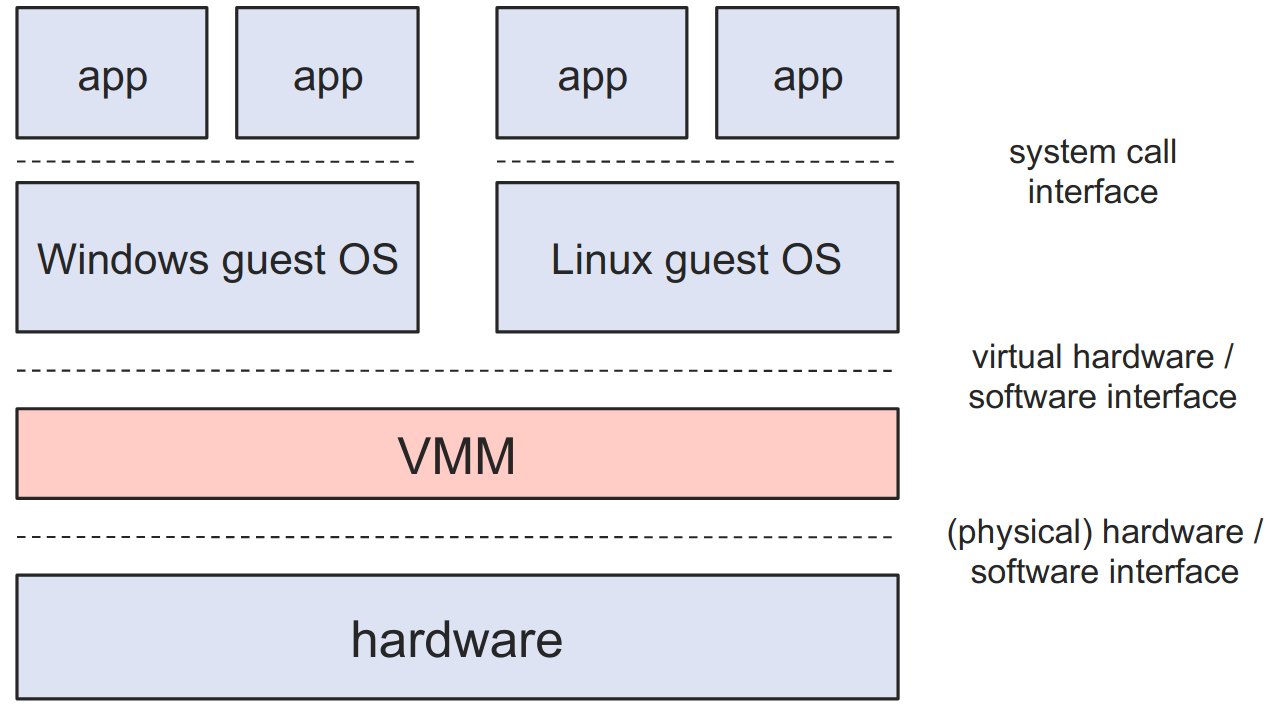
\includegraphics[width=1.\textwidth]{vmm-do-work}
			
		\end{column}
		
		\begin{column}{.8\textwidth}
			
			%			What if we run the Linux/Windows kernel as a user-level program?	
			
			\centering
			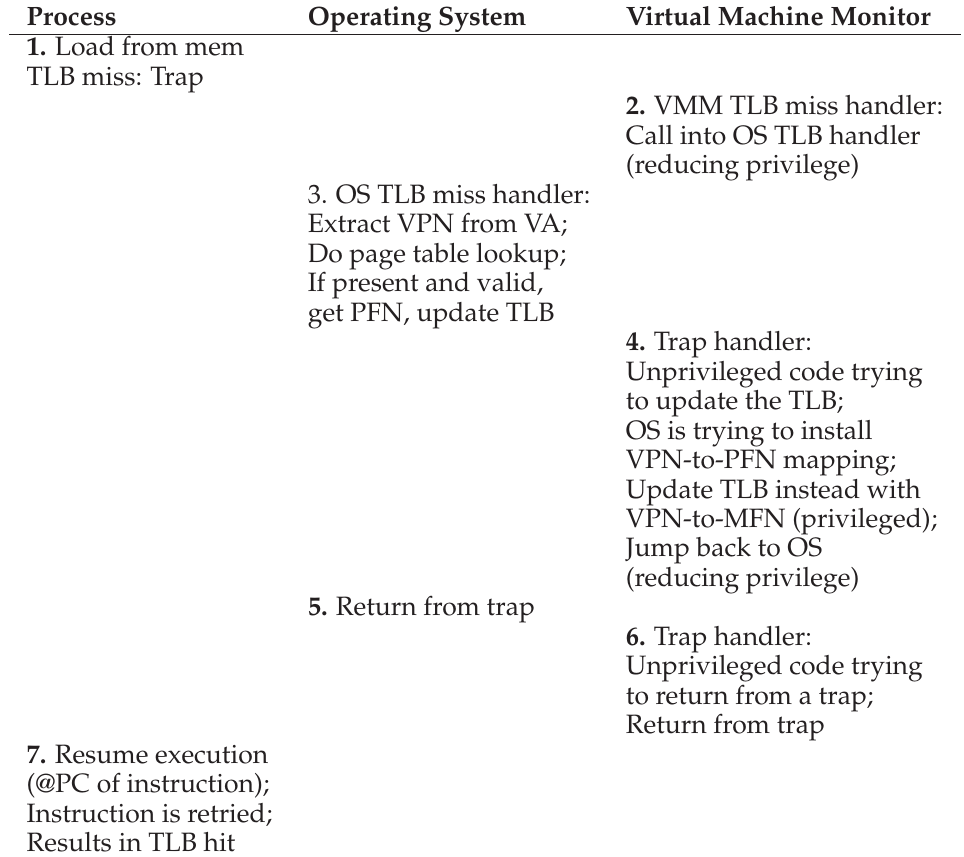
\includegraphics[width=.65\textwidth]{vmm-tlbmiss}	
			%			\begin{flushleft}
			
			TLB Miss Flow with Virtualization
			
			%			\end{flushleft}
			
			
		\end{column}
		
		
	\end{columns}
	
	
\end{frame}

%-------------------------------------------------
\begin{frame}[plain]
	\frametitle{How VMM works -- memory}
	
	
	
	\begin{columns}
		
		\begin{column}{.4\textwidth}
			\centering
			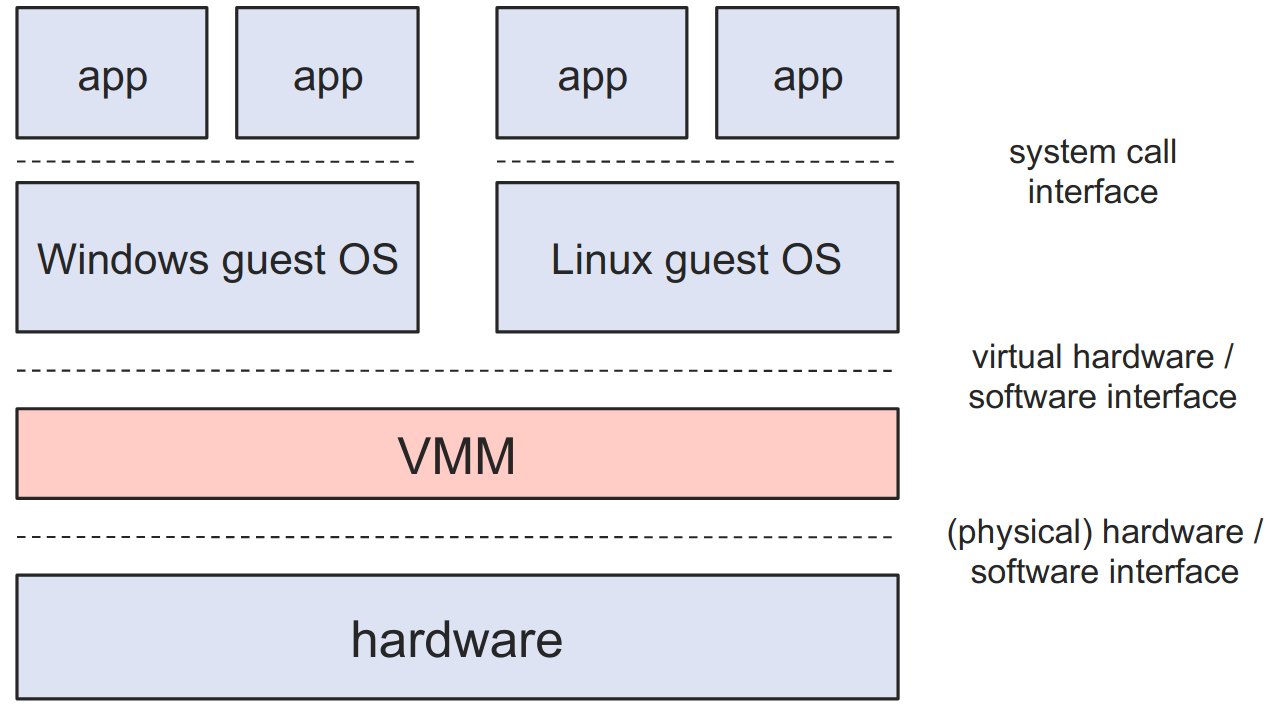
\includegraphics[width=1.\textwidth]{vmm-do-work}
			
		\end{column}
		
		\begin{column}{.6\textwidth}
			
			 How does the virtual machine monitor get involved with a
			hardware-managed TLB?	
			
			\begin{itemize}
				\item VMM doesn't have a chance to run on each TLB miss to sneak its translation into the system. 
				\item VMM must closely monitor changes	the OS makes to each page table
				\item VMM must keep a \textbf{shadow page table} that maps the virtual addresses of each process to the VMM's desired machine pages
				\item VMM installs a process's \textbf{shadow page table }whenever the OS tries to install the process's	OS-level page table
				
			\end{itemize} 

			
			
		\end{column}
		
		
	\end{columns}
	
	
\end{frame}


%-------------------------------------------------
\begin{frame}[plain]
	\frametitle{How VMM works -- memory}
	
	
	
	\begin{columns}
		
		\begin{column}{.4\textwidth}
			\centering
			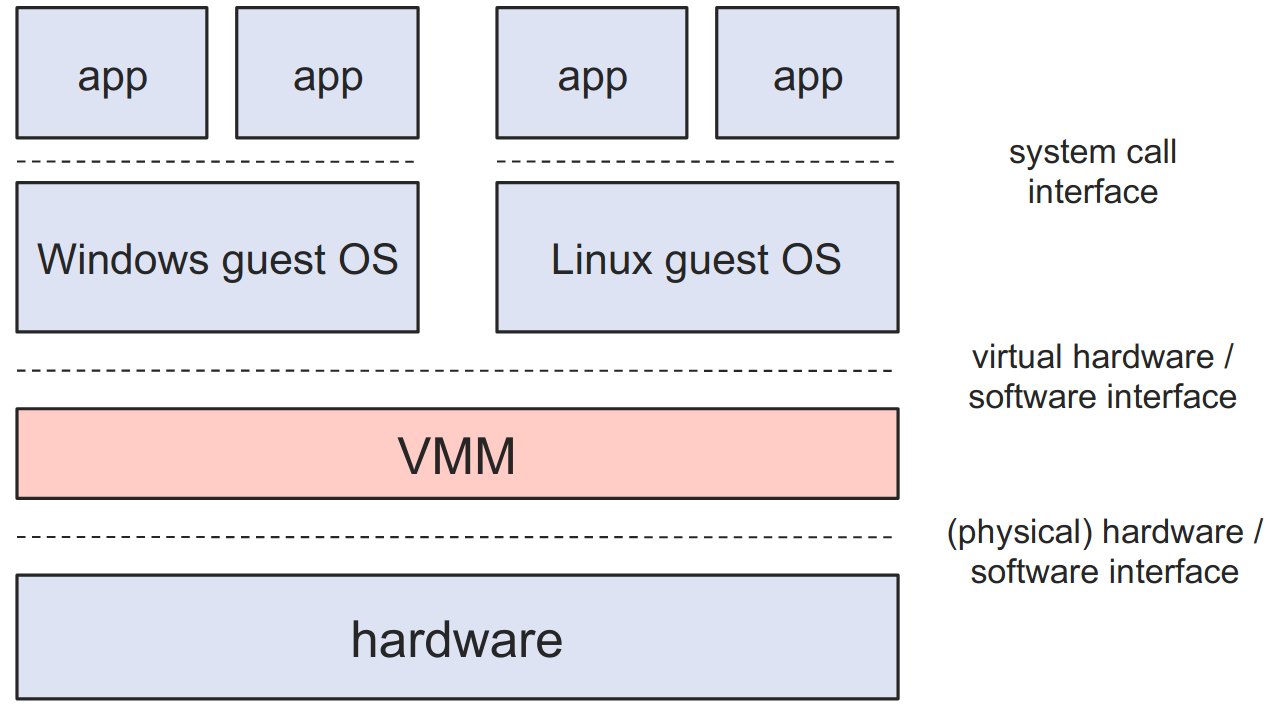
\includegraphics[width=1.\textwidth]{vmm-do-work}
			
		\end{column}
		
		\begin{column}{.6\textwidth}
			
			How does the virtual machine monitor get involved with a
			hardware-managed TLB?	
			
			\begin{itemize}
				\item VMM doesn't have a chance to run on each TLB miss to sneak its translation into the system. 
				\item VMM must closely monitor changes	the OS makes to each page table
				\item VMM must keep a \textbf{shadow page table} that maps the virtual addresses of each process to the VMM's desired machine pages
				\item VMM installs a process's \textbf{shadow page table }whenever the OS tries to install the process's	OS-level page table
				
			\end{itemize} 
			
			
			
		\end{column}
		
		
	\end{columns}
	
	
\end{frame}


%-------------------------------------------------
\begin{frame}[plain]
	\frametitle{How VMM works -- IO}
	
	
	
	\begin{columns}
		
		\begin{column}{.4\textwidth}
			\centering
			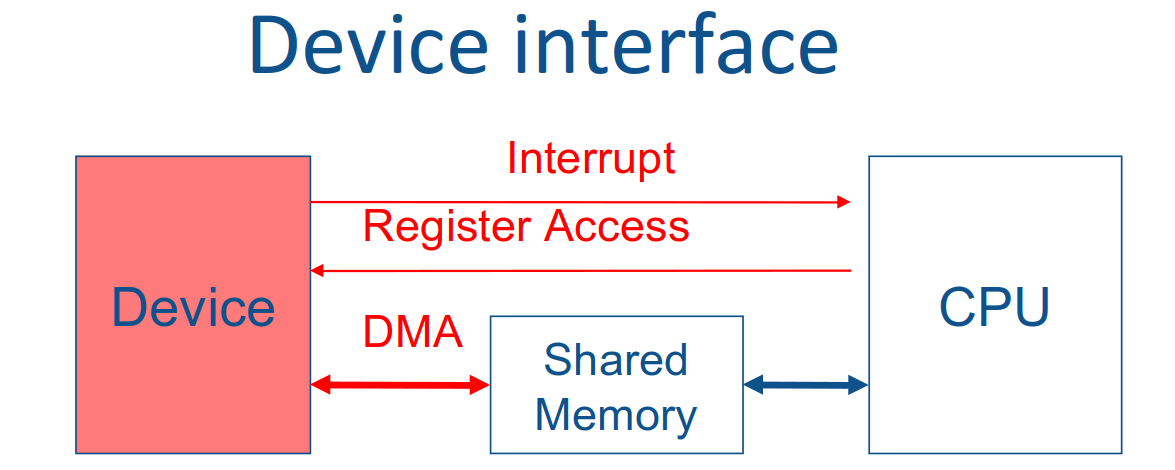
\includegraphics[width=1.\textwidth]{device-interface}
			
		\end{column}
		
		\begin{column}{.6\textwidth}
			
		\begin{itemize}
			\item Interaction between device and driver:
			\begin{itemize}
				\item Driver programs device through register access 
				\item Device notifies driver through interrupt
				\item Device could DMA for massive data movement
				
			\end{itemize} 
		
	  \end{itemize} 	
			
			
		\end{column}
		
		
	\end{columns}
	
	
\end{frame}


%-------------------------------------------------
\begin{frame}[plain]
	\frametitle{How VMM works -- IO}
	
	
	
	\begin{columns}
		
		\begin{column}{.4\textwidth}
			\centering
			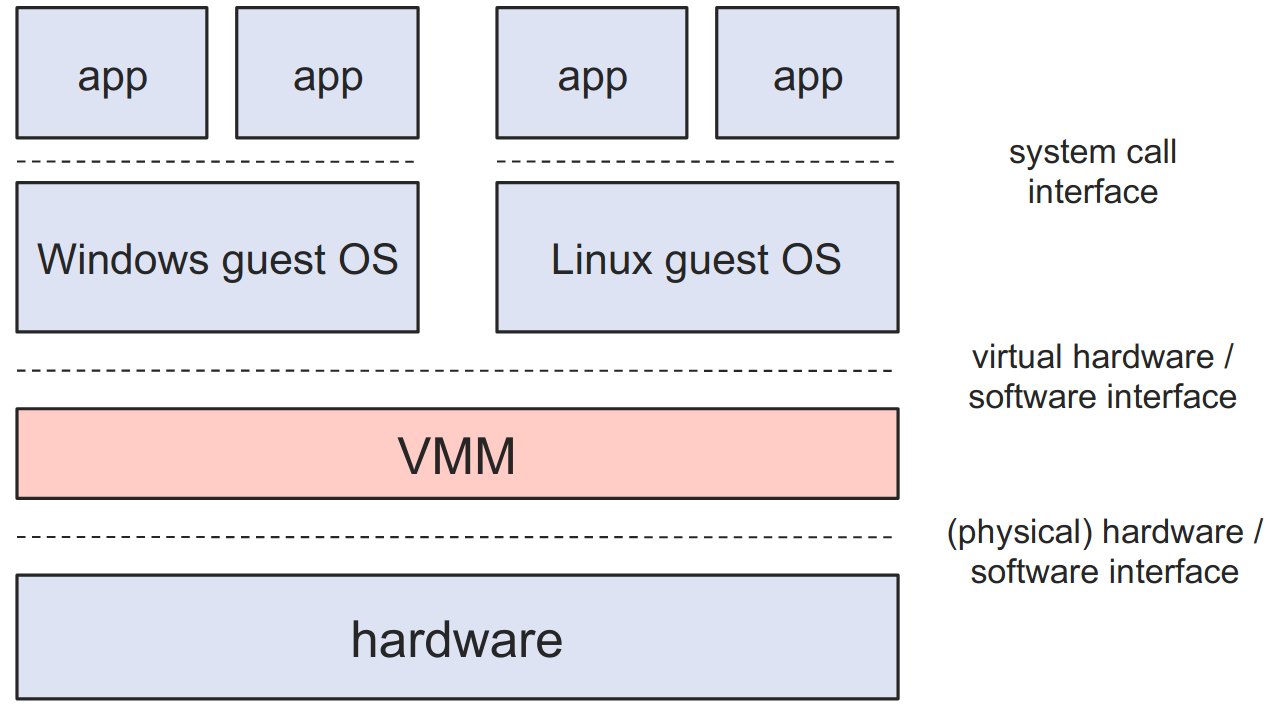
\includegraphics[width=1.\textwidth]{vmm-do-work}
			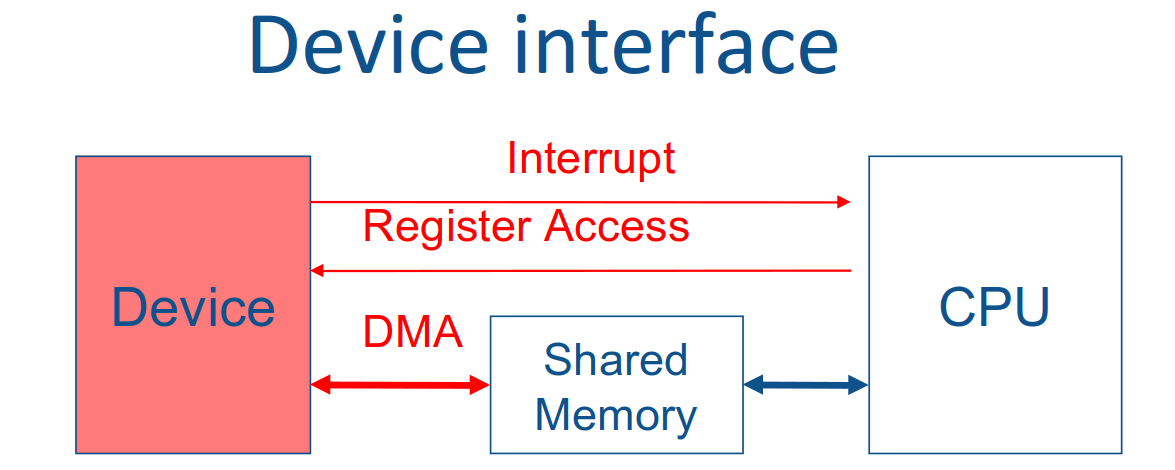
\includegraphics[width=1.\textwidth]{device-interface}
		\end{column}
		
		\begin{column}{.6\textwidth}
			
			\begin{itemize}
				\item I/O Virtualization requires the hypervisor to present guest a complete device interface
				\begin{itemize}
					\item Presenting an existing interface: Software Emulation
					\item Presenting an existing interface: Direct assignment
					
				\end{itemize} 
				\item Presenting a brand new interface
				\begin{itemize}
					\item Paravirtualization
					
				\end{itemize} 
			\end{itemize} 	
			
			
		\end{column}
		
		
	\end{columns}
	
	
\end{frame}

%-------------------------------------------------
\begin{frame}[plain]
	\frametitle{How VMM works -- IO}
	
	
	
	\begin{columns}
		
		\begin{column}{.4\textwidth}
			\centering
			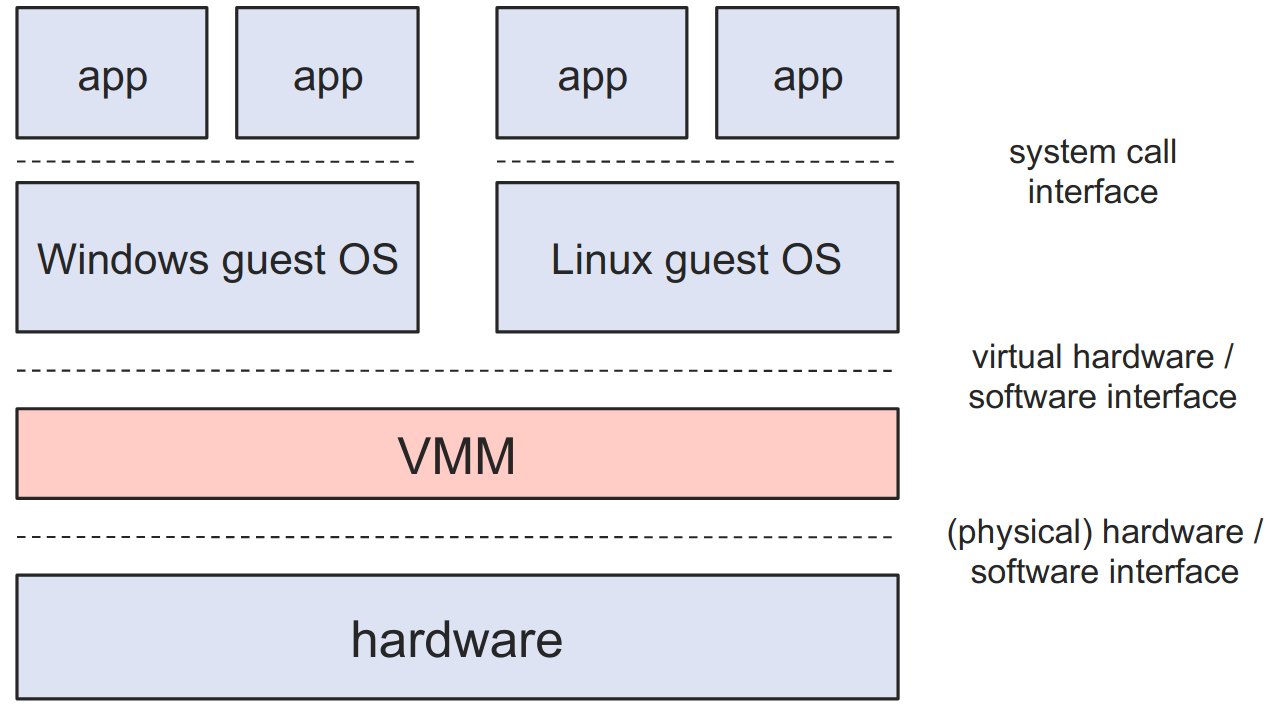
\includegraphics[width=.8\textwidth]{vmm-do-work}
			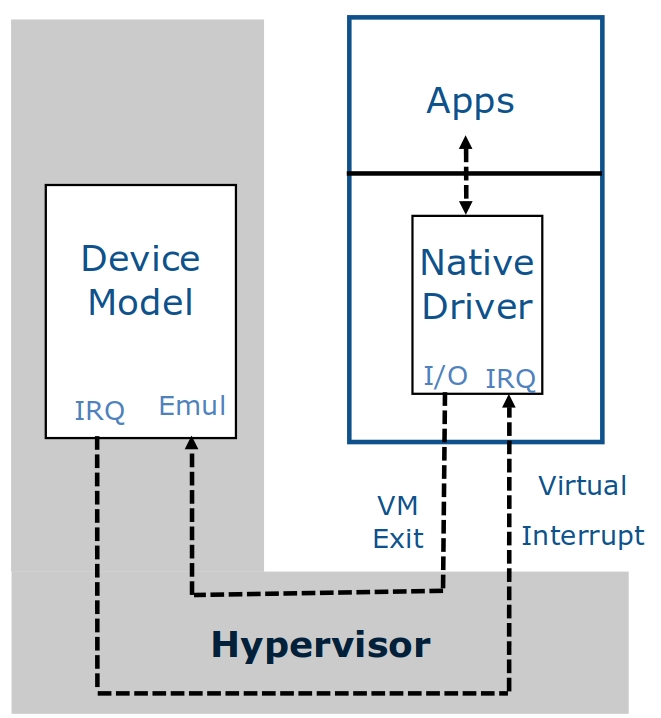
\includegraphics[width=.7\textwidth]{vmm-io-soft-emulation}
		\end{column}
		
		\begin{column}{.6\textwidth}
			Software Emulation
			\begin{itemize}
				\item Guest runs native device driver, e.g. NE2000
				\begin{itemize}
					\item I/O access is trap-and-emulated by device model in hypervisor
					\item Translation for MMIO is zapped
					\item Virtual Interrupt is signaled by device model per semantics
					
				\end{itemize} 
				\item Excessive trap and emulation

			\end{itemize} 	
			
			
		\end{column}
		
		
	\end{columns}
	
	
\end{frame}

%-------------------------------------------------
\begin{frame}[plain]
	\frametitle{How VMM works -- IO}
	
	
	
	\begin{columns}
		
		\begin{column}{.4\textwidth}
			\centering
			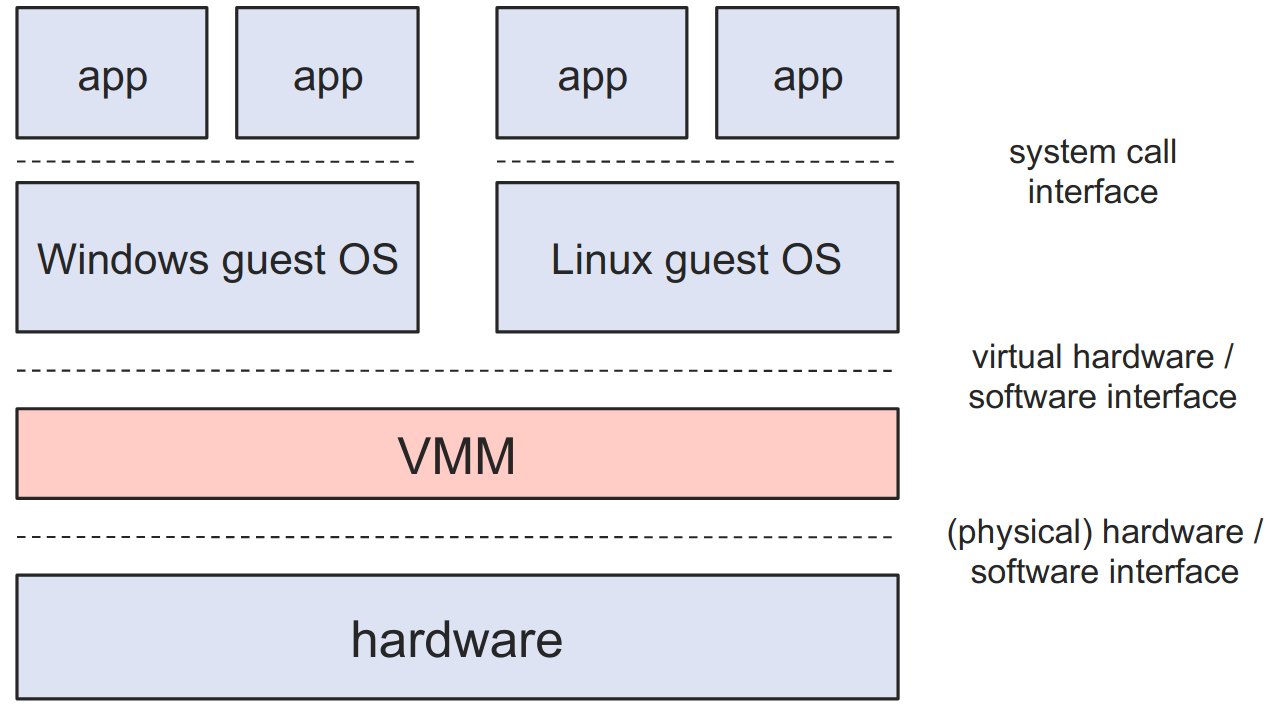
\includegraphics[width=.8\textwidth]{vmm-do-work}
			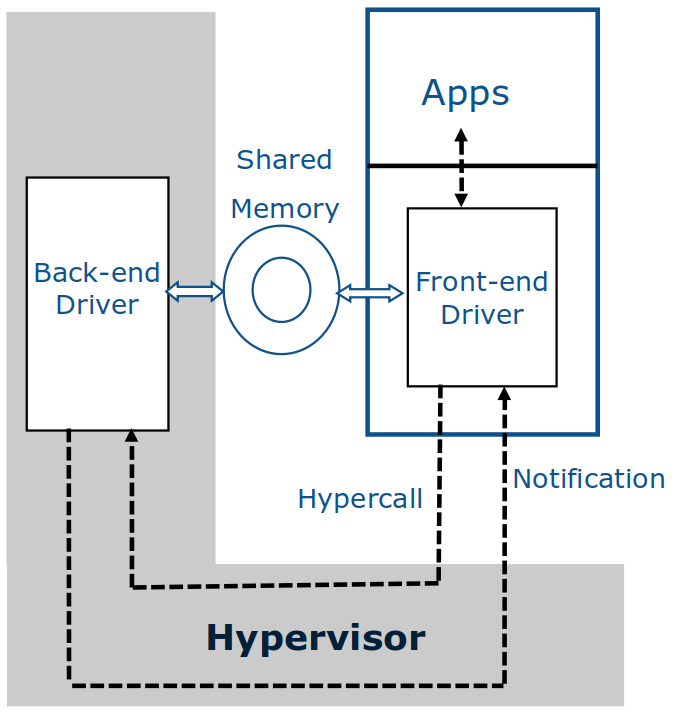
\includegraphics[width=.7\textwidth]{vmm-io-paravirt}
		\end{column}
		
		\begin{column}{.6\textwidth}
			Paravirtualization
			\begin{itemize}
				\item A new front-end driver (FE driver) is run in guest
				\begin{itemize}
					\item Optimized request through hypercall
					
				\end{itemize} 
			
				\item Hypervisor runs a back-end driver (BE driver) to service request from FE driver
				\begin{itemize}
					\item Notify guest for processing
	
				\end{itemize} 			
			
			\item Shared memory is used for massive data communication
			\begin{itemize}
				\item To reduce guest/hypervisor boundary crossin
				\item e.g. Xen VNIF, KVM Virtio-Net
			\end{itemize} 
			
			\end{itemize} 	
			
			
		\end{column}
		
		
	\end{columns}
	
	
\end{frame}
%-------------------------------------------------
%-------------------------------------------------


\end{document}